%:Clase del documento
\documentclass[fontsize=10pt, Myfinal=true, twoside, numbers=noenddot]{scrbook}
%Minion=true, English=true, Myfinal=true

%:Paquete de estilos propuesto
\usepackage{libroETSI}

%:Paquete específico para cargar tikz (y sus librerías) y pgfplots
\usepackage{dtsc-creafig}

%:Paquete para notaciones específicas
\usepackage{notacion}

%:Paquete para incorporar aspectos concretos de la edición
\usepackage{edicionPFC}


%:Estas líneas de código son INNECESARIAS excepto para mostrar determinadas características en este manual. Pueden eliminarse o comentarse sin ningún problema.
%Se usan para compilar el capítulo estilolibroetsi.tex
\usepackage[final]{showexpl}
\lstset{explpreset={frame=none,rframe={}, numbers=none,numbersep=3pt, columns=flexible,language={[LaTeX]TeX},basicstyle=\ttfamily,keywordstyle=\color{blue}}}%numberstyle=\tiny,

%:Para modificar fácilmente la fuente del texto.
\makeatletter
\ifdtsc@Minion % Queremos utilizar la fuente Minion y lo hemos declarado al principio
	\ifluatex
		\setmainfont[Renderer=Basic, Ligatures=TeX,	% Fuente del texto 
		Scale=1.01,
		]{Minion Pro}
   		% En este caso conviene modificar ligeramente el tamaño de las fuentes matemáticas
		\DeclareMathSizes{10}{10.5}{7.35}{5.25}
		\DeclareMathSizes{10.95}{11.55}{8.08}{5.77}
		\DeclareMathSizes{12}{12.6}{8.82}{6.3}
%		\setmainfont[Renderer=Basic, Ligatures=TeX,	% Fuente del texto 
%		]{Adobe Garamond Pro}
%		\setmainfont[Renderer=Basic, Ligatures=TeX,	% Fuente del texto 
%		]{Palatino LT Std}
	\fi
\else
	\ifluatex
		% Para utilizar la fuente Times New Roman, o alguna otra que se tenga instalada
		\setmainfont[Renderer=Basic, Ligatures=TeX,	% Fuente del texto 
		Scale=1.0,
		]{Times New Roman}
	\else
		\usepackage{tgtermes} 	%clone of Times
		%\usepackage[default]{droidserif}
		%\usepackage{anttor} 	
	\fi
\fi
\makeatother

%Por si quieren usar bibliografía con BIBER
%BIBER%%:Para la bibliografía en BIBER, descomentar las líneas siguientes
%\defbibheading{etsi}[]{%
%	\chapter*{Bibliografía}%
%	\chaptermark{Bibliografía} 
%	\markboth{#1}{#1}}
%\addbibresource{bibliografiaLibroETSI.bib}

% Ejemplo de Glosario
\newacronym[type=main]{ETSI}{ETSI}{Escuela Técnica Superior de Ingeniería}
\newacronym[type=main]{US}{US}{Universidad de Sevilla}
\newacronym[type=main]{PDI}{PDI}{Polidispersity Index}


\makeindex
\makeglossaries %Si no se quiere el glosario, comentar esta línea.

% Formato A4
\geometry
{paperheight=297mm,%
paperwidth=210mm,%
top=25mm,%
headsep=8.5mm,%
includefoot, 
textheight=240mm, 
textwidth=150mm, 
bindingoffset=0mm, 
twoside}

\usepackage[a4,center]{crop}%para poner las cruces de esquina de página, poner la opción cross

%:Esquema de numeración por defecto
\setenumerate[1]{label=\normalfont\bfseries{\arabic*.}, leftmargin=*, labelindent=\parindent}
\setenumerate[2]{label=\normalfont\bfseries{\alph*}), leftmargin=*}
\setenumerate[3]{label=\normalfont\bfseries{\roman*.}, leftmargin=*}
\setlist{itemsep=.1em}
\setlength{\parindent}{1.0 em}

\setcounter{tocdepth}{4}						% El nivel hasta el que se muestra el índice 


%:Empieza el documento

\begin{document}
%:Para incluir toda la referencia bibliográfica aunque no se cite, descomente la siguiente línea
%\nocite{*}


%PORTADA
%ver edicionPFC.sty para modificaciones

%:Para crear la portada y la portada interior (pagina titular)
\titulo{Produccion masiva de microburbujas monodispersas para aplicaciones reales evitando la microfluídica} %\mbox evita que se divida una palabra al cambiar de línea
\autor{Enrique J. Sánchez Quintero}
\director{José Manuel Gordillo Arias de Saavedra}
\titulodirector{Catedrático de Universidad}

\departamento{Dep. Mecánica de Fluidos e Ingeniería Aeroespacial}
\centro{Escuela Técnica Superior de Ingeniería}
\universidad{Universidad de Sevilla}
\titulacion{Máster de Diseño Avanzado en Ingeniería Mecánica}
\fecha{2017}
\nombretrabajo{Trabajo Fin de Máster} %Trabajo Fin de Grado, Proyecto fin de Máster,....

\hypersetup
	{
 	linkcolor=black, %Tocar para poner color en enlaces
	pdfauthor={\elautor},
	pdftitle={\nombretrabajo,\eltitulo}, 
	pdfkeywords={Latex, edición, formato de texto}	
	 }

\portadaPFC{figuras/LogoUS.pdf}{figuras/LogoTSC.pdf} %logo de la Universidad y logo del departamento, si lo hubiera. Para cambiar el pie de página con los logos, debe editarse el fichero ediciónPFC.sty

%Fin Portada

%:Todo lo que constituye la primera parte del libro que no es el cuerpo del libro en realidad
\frontmatter
\pagenumbering{Roman} %Pone la numeración en mayúscula (En español parece que es obligatorio)

%\include{dedicatoria/dedicatoria}%¿Comentar para proyectos/tesis?
% !TEX root =../LibroTipoETSI.tex
\chapter*{Agradecimientos}
%\pagestyle{especial}
\pagestyle{empty}
%\chaptermark{Agradecimientos}
\phantomsection
%\addcontentsline{toc}{listasf}{Agradecimientos}
%\vspace{1cm}
%{\huge{Agradecimientos}}
%\vspace{1cm}

\lettrine[lraise=-0.1, lines=2, loversize=0.25]{E}{l} diseño de una hoja de estilo en \LaTeX\ para un texto no es en absoluto trivial. Por un lado hay que conocer bien los usos, costumbres y reglas que se emplean a la hora de establecer márgenes, tipos de letras, tamaños de las mismas, títulos, estilos de tablas, y un sinfín de otros aspectos. Por otro, la programación en \LaTeX\ de esta hoja de estilo es muy tediosa, incluida la selección de los mejores paquetes para ello. La hoja de estilo adoptada por nuestra Escuela y utilizada en este texto es una versión de la que el profesor Payán realizó para un libro que desde hace tiempo viene escribiendo para su asignatura. Además, el prof. Payán ha participado de forma decisiva en la adaptación de dicha plantilla a los tres tipos de documentos que se han tenido en cuenta: libro, tesis y proyectos final de carrera, grado o máster. Y también en la redacción de este texto, que sirve de manual para la utilización de estos estilos. Por todo ello, y por hacerlo de forma totalmente desinteresada, la Escuela le está enormemente agradecida.

A esta hoja de estilos se le incluyó unos nuevos diseños de portada. El diseño gráfico de las portadas para proyectos fin de grado, carrera y máster, está basado en el que el prof. Fernando García García, de la Facultad de Bellas Artes de nuestra Universidad, hiciera para los libros, o tesis, de la sección de publicación de nuestra Escuela. Nuestra Escuela le agradece que pusiera su arte y su trabajo, de forma gratuita, a nuestra disposición.

%gradecemos}, a todos nuestros maestros, cuanto nos enseñaron.

{\flushleft{\hfill \emph{Juan José Murillo Fuentes}}}%
\vspace{-.3cm}
{\flushleft{\hfill \emph{Subdirección de Comunicaciones y Recursos Comunes}}}%
{\flushleft{\hfill \emph{Sevilla, 2013}}}%

%PFC/PFM/TESIS
% !TEX root =../LibroTipoETSI.tex
\chapter*{Resumen}
\pagestyle{especial}
\chaptermark{Resumen}
\phantomsection
\addcontentsline{toc}{listasf}{Resumen}

\lettrine[lraise=-0.1, lines=2, loversize=0.2]{E}{n} nuestra Escuela se producen un número considerable de documentos, tantos docentes como investigadores. Nuestros alumnos también contribuyen a esta producción a través de sus trabajos de fin de grado, máster y tesis. El objetivo de este material es facilitar la edición de todos estos documentos y a la vez fomentar nuestra imagen corporativa, facilitando la visibilidad y el reconocimiento de nuestro Centro.

%La hoja de estilo utilizada es una versión de la que el Prof. Payán realizó para un libro que desde hace tiempo viene escribiendo para su asignatura. Con ella se han realizado estas notas, a modo de instrucciones, añadiéndole el diseño de la portada. El diseño de la portada está basado en el que el prof. Fernando García García, de nuestra universidad, hiciera para los libros de la sección de publicación de nuestra Escuela.


\chapter*{Abstract}
\pagestyle{especial}
\chaptermark{Abstract}
\phantomsection
\addcontentsline{toc}{listasf}{Abstract}

\lettrine[lraise=-0.1, lines=2, loversize=0.2]{I}{n} our school there are a considerable number of documents, many teachers and researchers. Our students also contribute to this production through its work in order of degree, master's theses. The aim of this material is easier to edit these documents at the same time promote our corporate image, providing visibility and recognition of our Center. 

...
\emph{-translation by google-}

 

% Índice abreviado 
% El índice abreviado se incluye también en algunos libros, con menor detalle que el completo. Descomentar las siguientes líneas.
\cleardoublepage
\phantomsection
\addcontentsline{toc}{listasf}{Índice Abreviado}
\pagestyle{especial}
\shorttoc{Índice Abreviado}{1}

%Índice normal, el completo
\cleardoublepage
\phantomsection
\pagestyle{especial}
\tableofcontents


%:---------------------------Notación 
%Toda esta notación es opcional, pero creemos que puede ser de mucha ayuda.
%Juan José Murillo Fuentes y Javier Payán Somet. Copyright 2011. Todos los derechos reservados.

%:---------------------------------------------------  Referencias
%Puede usar los comandos \label y \ref, pero con lo de abajo se facilita el uso de múltiples etiquetas para ecuaciones, secciones,...
%Etiquetas:
\newcommand{\LABEQ}[1]{\label{eq:#1}}%\mathtt{[eq:#1]}\qquad %Equación
\newcommand{\LABALG}[1]{\label{alg:#1}}%\mathtt{[lab:#1]}\qquad %Algoritmo
\newcommand{\LABTAB}[1]{\label{tab:#1}}%{\tt [tab:$\text{$#1$}$]}} %Tabla
\newcommand{\LABFIG}[1]{\label{fig:#1}}%{\tt [fig:$\text{$#1$}$]}} %Figura
\newcommand{\LABTHM}[1]{\label{thm:#1}}%{\tt [thm:#1]}} % Teorema
\newcommand{\LABPRP}[1]{\label{prp:#1}}%{\tt [prp:#1]}} % Proposición
\newcommand{\LABLEM}[1]{\label{lem:#1}}%{\tt [lem:#1]}} % Lema
\newcommand{\LABCOR}[1]{\label{cor:#1}}%{\tt [cor:#1]}} %Corolario 
\newcommand{\LABDFN}[1]{\label{dfn:#1}}%{\tt [dfn:#1]}} %Definición
%\newcommand{\LABFNT}[1]{\label{fnt:#1}}%{\tt [fnt:#1]}} %
%
%Referencias a las etiquetas anteriores, Incluyen el título. Puede cambiarlos aquí. Por ejemplo, si quiere "Fig." en vez de "Figura"...
\newcommand{\EQ}[1]{Ecuación~\eqref{eq:#1}}%$^{\text{\tt [#1]}}$} %used to be {(\ref{eq:#1})}
\newcommand{\ALG}[1]{~\ref{alg:#1}}
\newcommand{\TAB}[1]{Tabla ~\ref{tab:#1}}%$^{\text{\tt [#1]}}$}
%\newcommand{\TAB}[1]{\autoref{tab:#1}}%$^{\text{\tt [#1]}}$}
\newcommand{\FIG}[1]{Figura~\ref{fig:#1}} %$^{\text{\tt [#1]}}$} 
%\newcommand{\FIG}[1]{\autoref{fig:#1}} %$^{\text{\tt [#1]}}$} 

%\newcommand{\FIG}[1]{Fig. \ref{fig:#1}} %$^{\text{\tt [#1]}}$} 
\newcommand{\THM}[1]{Teorema~\ref{thm:#1}}%$^{\text{\tt [#1]}}$}
\newcommand{\COR}[1]{Corolario~\ref{cor:#1}}%$^{\text{\tt [#1]}}$}
\newcommand{\PRP}[1]{Propiedad~\ref{prp:#1}}%$^{\text{\tt [#1]}}$}
\newcommand{\LEM}[1]{Lema~\ref{lem:#1}}%$^{\text{\tt [#1]}}$}
\newcommand{\DFN}[1]{Definición~\ref{dfn:#1}}%$^{\text{\tt [#1]}}$}
%\newcommand{\FNT}[1]{~\ref{fnt:#1}}%$^{\text{\tt [#1]}}$}

%Etiquetas para títulos tipo capítulo, sección, subsección,...
\newcommand{\LABCHAP}[1]{\label{chap:#1}}%{\tt [chap:#1]}}
\newcommand{\LABAPEN}[1]{\label{apen:#1}}%{\tt [chap:#1]}}
\newcommand{\LABSEC}[1]{\label{sec:#1}}%{\tt [sec:#1]}}
\newcommand{\LABSSEC}[1]{\label{ssec:#1}}%{\tt [ssec:#1]}}
\newcommand{\LABSSSEC}[1]{\label{sssec:#1}}%{\tt [sssec:#1]}}
%
%Referencias para los anteriores títulos
\newcommand{\CHAP}[1]{Capítulo~\ref{chap:#1}}%$^{\text{\tt [c:#1]}}$}
\newcommand{\SEC}[1]{Sección~\ref{sec:#1}}%$^{\text{\tt [s:#1]}}$}
\newcommand{\SSEC}[1]{Subsección~\ref{ssec:#1}}%$^{\text{\tt [ss:#1]}}$}
\newcommand{\SSSEC}[1]{Apartado~\ref{sssec:#1}}%$^{\text{\tt [sss:#1]}}$}
\newcommand{\APEN}[1]{Apéndice~\ref{apen:#1}}%$^{\text{\tt [c:#1]}}$}
%
%%
%\newcommand{\PAGEEQ}[1]{~\pageref{eq:#1}}
%\newcommand{\PAGETAB}[1]{~\pageref{tab:#1}}
%\newcommand{\PAGEFIG}[1]{~\pageref{fig:#1}}


%%%%Definiendo caligrafías especiales 
%\newcommand{\emphb}[1]{\emph{\textbf{#1}}}
%\newcommand{\X}{\calg{X}} %{\ensuremath{\calg{X}}} %\textrm{\ifmmode {1pt} \else {\, } \fi}
%\newcommand{\Y}{\calg{Y}}%{\ensuremath{\calg{Y}}}
\newcommand{\calg}[1]{\ensuremath{\mathcal{#1}}} %JJMF: No entiendo para qué es esto.
%\newcommand{\hb}[1]{\ensuremath{\textrm{\usefont{T1}{phv}{b}{n}#1}}}
%\newcommand{\hn}[1]{\ensuremath{\textrm{\usefont{T1}{phv}{m}{n}#1}}}

%
%:Renombrando overline
%\newcommand{\overl}[1]{\bar{#1}}

\DeclarePairedDelimiter\ceil{\lceil}{\rceil}
\DeclarePairedDelimiter\floor{\lfloor}{\rfloor}

%%%% vectores
%
\newcommand{\vect}[1]{\mathbf{#1}}     %vectors (bold type)
\newcommand{\vc}[1]{\mathbf{#1}}     %vectors (bold type)
\newcommand{\matr}[1]{\mathbf{#1}}     %matrices (bold type)
% ó:
%\newcommand{\vc}[1]{\ensuremath{\mathbf{#1}}}
% ó:
%\newcommand{\vct}[1]{\boldsymbol{#1}}
%\newcommand{\vect}[1]{\boldsymbol{#1}}  %vectors (bold type)
%\newcommand{\matr}[1]{\boldsymbol{#1}}  %matrices (bold type)

\renewcommand*{\j}{\ensuremath{\textrm{j}}}%{\mathop{}\mathrm{j}}

%%%% Complejos y exponenciales
\newcommand{\xp}[1]{\e^{\j{#1}}}         %simple exponential
\newcommand{\xppi}[1]{\e^{\j2\pi{#1}}}         %simple exponential
\newcommand{\nxp}[1]{\e^{-\j{#1}}}       %negative exponential
\newcommand{\nxppi}[1]{\e^{-\j2\pi{#1}}}       %negative exponential
\newcommand{\e}{\mathrm{e}}
%\newcommand{\xp}[1]{\e^{j{#1}}}         %simple exponential
%\newcommand{\nxp}[1]{\e^{-j{#1}}}       %negative exponential
%
%
% Parte real
\newcommand{\re}{\mbox{$\mathrm{I\!Re}$}}       %real part
%\renewcommand{\Re}{\ensuremath{\boldsymbol{\mathcal{R}}}}
%\renewcommand{\Re}{\ensuremath{\textrm{\usefont{T1}{phv}{m}{n}Re}}}
% Parte imaginaria
\newcommand{\im}{\mbox{$\mathrm{I\!Im}$}}       %imaginary part
%\renewcommand{\Im}{\ensuremath{\boldsymbol{\mathcal{I}}}}
%\renewcommand{\Im}{\ensuremath{\textrm{\usefont{T1}{phv}{m}{n}Im}}}
%:Creando la unidad imaginaria
%\renewcommand{\j}{\ensuremath{\textrm{\usefont{T1}{lmr}{m}{n}j}}}


%%%% Maths functions and symbols
%
%:Para definir funciones matemáticas en castellano
\makeatletter
\ifdtsc@English
	\DeclareMathOperator{\sen}{sin}
	\DeclareMathOperator{\tg}{tg}  %tg() function
	\DeclareMathOperator{\arctg}{arctg}     %arctg() function
\fi
\makeatother

\DeclareMathOperator{\sa}{Sa}
%
\DeclareMathOperator{\sgn}{sgn}
%\newcommand{\sgn}{\mathrm{sign}}        %sign() function
%\newcommand{\sign}{\mathrm{sign}}
%
\DeclareMathOperator{\rect}{rect}
\DeclareMathOperator{\sinc}{Sinc}
%\newcommand{\cost}{\psi}                %cost or contrast function
\newcommand{\pder}[2]{\frac{\partial #1}{\partial #2}}  %partial derivative
%
%
%\renewcommand{\mod}{\bmod}      %\:\text{mod}\:}
\newcommand{\RR}{\mathbb{R}}            %real numbers
\newcommand{\CC}{\mathbb{C}}    %complex numbers
%
%\newcommand{\tg}{\mahtrm{tg}}           
%\newcommand{\angl}{\arg}
%
\newcommand{\costo}[2]{\cos^{#1}\!#2}   %cos to power
\newcommand{\sento}[2]{\sin^{#1}\!#2}   %sen to power
%
\newcommand{\gra}{\ensuremath{^\circ}}  %Grados. Ejemplo: $5\gra$ K serían 5º K


%%%% Matrices, traspuesta, hermítica, ...
%
\newcommand{\inv}{^{-1}}                %inverse operator
\newcommand{\trs}{^\top}                %transposition operator
%\newcommand{\trs}{^{\textrm{\usefont{T1}{phv}{b}{n}{T}}}}          %transponer una matriz
\newcommand{\psd}{^\dagger}             %pseudoinverse operator
\newcommand{\cnj}{^*}                   %complex conjugate
\newcommand{\pcnj}{^{\phantom{*}}}      %phantom complex conjugate (for alignment)
\newcommand{\her}{^\mathrm{H}}          %complex conjugate transpose
%\newcommand{\her}{^{\textrm{\usefont{T1}{phv}{b}{n}{H}}}}          %Hermítica
\newcommand{\id}[1]{\vect{I}_{#1}}       %identity matrix
%\newcommand{\id}{\matr{I}}       %identity matrix
\newcommand{\diag}[1]{\mathrm{diag}\left(#1\right)}     %diagonal
%\DeclareMathOperator{\diag}{diag}



%%%% indices de prestaciones %%%%%%%%%
%
%\newcommand{\isr}{\mathrm{ISR}}           %interference-to-signal ratio
\newcommand{\snr}{\mathrm{SNR}}           %signal-to-noise ratio
\newcommand{\mse}{\mathrm{MSE}}           %minimum mean square error
%
%ó se pueden escribir como
%\newcommand{\SNR}{\ensuremath{\textrm{SNR}}}
%...


%%%%Miscellaneos
%
%Redefiniendo epsilon
%\renewcommand{\epsilon}{\ensuremath{\textrm{\usefont{OML}{cmr}{m}{n}\symbol{15}}}}
%
%:Creando ``tal que'' de las expresiones matemáticas
\newcommand{\talq}{\colon}
%
%%Creando ``igual por definición'' de las expresiones matemáticas
\newcommand{\eqdef}{\ensuremath{\mathrel{\stackrel{\mathrm{def}}{=}}}}
%%ó
%\newcommand{\eqdef}{\triangleq}         %equal by definition
%
%
%:Creando la igualdad basada en una ecuación
%\newcommand{\igualref}[1]{\ensuremath{\mathrel{\stackrel{\mathrm{\eqref {#1}}}{=}}}}
%
%:Definiendo cardinal y norma
\newcommand{\norm}[1]{\ensuremath{\left\lVert #1 \right\rVert }}
\newcommand{\card}[1]{\ensuremath{\left| #1\right|}}
%\newcommand{\card}[1]{\ensuremath{\text{card}~#1}
%
%:Renombrando \boldsymbol
%\newcommand{\bm}[1]{\boldsymbol{#1}}
%
%:Facilitando la escritura de X_{i}
\newcommand{\xyz}[3]{\ensuremath{#1_{#2},#2=1,2,\ldots,#3}}
%
%:Creando el diferencial. Por defecto, dx
%\newcommand*{\df}[1][x]{\mathop{}\!\mathrm{d}{#1}}
\newcommand{\df}[1]{\mathrm{d}{#1}}

%
%%Modificando el menor igual y el mayor igual
\renewcommand{\le}{\leqslant}           %fancy \le
\renewcommand{\ge}{\geqslant}           %fancy \ge
%
%:Creando BL=backslash de las expresiones matemáticas
\newcommand{\BL}{\ensuremath{\backslash}}
%
%Redefiniendo iff
\renewcommand{\iff}{\Leftrightarrow}
%
%\newcommand{\what}{\widehat}
%\newcommand{\supp}[1]{^{(#1)}}          %superindex with parentheses
\newcommand{\eqexpl}[1]{\underset{#1}{\underset{\uparrow}{=}}}  %equal with explanation
%\newcommand{\proof}{\noindent {\bf Proof.} }
%\newcommand{\skproof}{\noindent {\bf Sketch of the proof.} }
\newcommand{\sfrac}[2]{\tfrac{#1}{#2}}  %small frac
\newcommand{\inc}{\Delta}
\newcommand{\ten}[1]{\cdot 10^{#1}}     %scientific notation
%\newcommand{\arrow}{$\rightarrow$ }
%\newcommand{\darrow}{$\Rightarrow$ }
%\newcommand{\tends}{\rightarrow}                         %'tends to'
\newcommand{\tendsub}[1]{\xrightarrow[#1]{}}             %{\underset{#1}{\longrightarrow}} %'tends to' with subscript
%\newcommand{\tendsubsup}[2]{\xrightarrow[#1]{#2}}        %{\overset{#2}{\tendsub{#1}}}   %'tends to' with sub and superscript
\newcommand{\ord}{\mathrm{O}}         %order of magnitude
\newcommand{\tm}{^{\text{\tiny{TM}}}} %trademark
%
%
%:Creando ``L'' de las expresiones matemáticas
%\renewcommand{\L}[1][L\!]{\ensuremath{\boldsymbol{\mathcal{#1}}}}
%\renewcommand{\L}[1][L\!]{\ensuremath{\boldsymbol{\mathscr{#1}}}}
%
%:Creando la F de transformada de Fourier
%\newcommand{\Fo}{\ensuremath{\boldsymbol{\mathscr{F}}}}
%
%:Creando la H de transformada de Hilbert
%\newcommand{\Hi}{\ensuremath{\boldsymbol{\mathscr{H}}}}
%
%
%%%% Indention
%
%\newcommand{\ind}{$\phantom{\indent}$}
%


%%%% Basic statistics
%
%%Creando el operador "valor esperado" 
%\newcommand{\E}{\ensuremath{\mathbb{E}}}
%\newcommand{\E}{\ensuremath{\textrm{\usefont{OML}{phv}{b}{n}E\hspace{1pt}}}}
%\newcommand{\E}{\ensuremath{\textrm{\usefont{T1}{phv}{m}{n}E}}}
\newcommand{\E}{\mathbb{E}}             %expected value
%
%%Definiendo el espacio de probabilidad
%\newcommand{\ep}{\ensuremath{\left( {\Omega, \calg{B}, \Pr} \right)}}
%\newcommand{\EP}{\ensuremath{\left( {\Omega, \calg{B}, \Pr} \right)}}
%
%\newcommand{\var}{\mathrm{Var}}         %variance
%\newcommand{\cov}{\mathrm{Cov}}         %covariance
\newcommand{\covm}[1]{\vc{C}_{#1}}           %covariance matrix
\newcommand{\corrm}[1]{\vc{R}_{#1}}           %correlation matrix
%\newcommand{\pdf}{p}                    %probability density function
%
%%Creando el operador "Probabilidad"
%\renewcommand{\Pr}{\ensuremath{\mathbb{P}}}
%\renewcommand{\Pr}{\ensuremath{\textrm{\usefont{T1}{phv}{m}{n}P}}}
%
%%Momentos
%\newcommand{\m}[1]{\mu_{#1}}            %moments
%\newcommand{\K}[1]{\kappa_{#1}}         %cumulants (symbol)
%\newcommand{\eK}[1]{\hat{\kappa}_{#1}}  %estimated cumulant
%\newcommand{\cum}{\mathrm{Cum}}         %cumulant
%\newcommand{\M}{\mathrm{M}}             %moment
%\newcommand{\C}{\mathrm{C}}             %cumulant (short)
%
%Creando la varianza
\newcommand{\si}[1]{\ensuremath{\sigma_{#1}^{2}}}
%
%Creando la expresión para indicar una gaussiana
\newcommand{\gauss}[2]{\ensuremath{\calg{N}\left( {#1, #2} \right)}}
%


%%Creando el espectro del ruido blanco
%\newcommand{\Sw}[1][W]{\ensuremath{S_{#1}\left( {\omega} \right)  = \frac{N_{0}}{2}}}
%\newcommand{\Sf}[1][W]{\ensuremath{S_{#1}\left( {\omega} \right)  = \frac{N_{0}}{2}}}
%\newcommand{\Swu}[1][W]{\ensuremath{S_{#1}\left( {\omega} \right)  = N_{0}/2} \textrm{w/(rad/s)}\finjps}
%\newcommand{\Sfu}[1][W]{\ensuremath{S_{#1}\left( {\omega} \right)  = N_{0}/2} \textrm{w/(Hz)}\finjps}
%
%%Creando el límite en el sentido de error cuadrático medio. Está copiado de amsopn.sty
%\def\lms{\qopname\relax m{l.i.m.}}
%
%%Creando el conjunto típico
%\newcommand{\ct}[1][T]{\ensuremath{#1_{\epsilon}^{n}}\ifmmode \else \ \fi}%[A]{\ensuremath{#1_{\epsilon}^{\left( {n} \right)}}}
%
%%Creando la función de distribución. Por defecto, F_{X}\left( {x} \right)
%\newcommand{\FD}[1][x]{\ensuremath{F_{\MakeUppercase{#1}}\left( \MakeLowercase{#1} \right)\ }}
%\newcommand{\FDP}{función de distribución\ }
%
%%Creando la función de densidad de probabilidad. Por defecto, f_{X}\left( {x} \right)
%\newcommand{\fd}[1][x]{\ensuremath{f_{\MakeUppercase{#1}}\left( \MakeLowercase{#1} \right)\ }}
%\newcommand{\fdp}{función densidad de probabilidad\ }



%%%% Revisiones
%
%\newcommand{\comentario}[1]{{\bf Comentario:} {\tt #1}?} 

%\newcommand{\cambiopor}[3]{\marginpar{\hfill{$\tendsubsup{#2}{\text{\tt #1}}$}} {\tt >>> #3}}
%
%\newcommand{\cambio}[2]{{{\tt #1}} {\tt >>> #2??}}
%
%\newcommand{\incluir}[1]{{\bf Incluir:} {\tt #1}?}
%\newcommand{\incluido}[1]{{\bf Incluido:} {\tt #1}}
%
%\newcommand{\notaFul}[1]{{\color{blue} {Fulano: \bf #1}}}



%%%%Ejemplo de notación típica
%
%\def\w{{\mathbf w}}        %GP Vector
%\def\r{{\mathbf r}}        %
%\newcommand{\PHI}{\boldsymbol{\Phi}}
%\def\b{{b}} %elemento de b
%\def\bve{{\mathbf \bve}}
%\def\d{{d}}
%\def\k{{ k}}
%\def\kk{{\mathbf \k}}
%\def\K{{\mathbf K}}
%\def\x{{\vect{x}}}
%\def\y{\vect{\b}}
%\def\newp{_{*}}        %GP Vector
%\def\newout{\b_{*}}
%\newcommand{\p}{\boldsymbol{\phi}}
%\def\X{{\mathbf X}}
%\def\teta{{\mathbf \theta}}
%\def\muw{{\mathbf \mu_\w}}
%\def\newin{{\vect{x}\subind{*}}}
%\def\fv{f}
%\def\fp{\vect{f}}
%
%\def\tset{\mathcal{D}}
%\def\mgp{\boldsymbol{\mu}}
%\def\Nor{\mathcal{N}}                %Gaussian distribution
%\def\treg{y} %Target value of a regression problem
%\def\tregnew{y_{*}}
%
%\ifluatex
%\makeatletter
%\DeclareRobustCommand{\LaTeX}{L\kern-.36em%
%        {\sbox\z@ T%
%         \vbox to\ht\z@{\hbox{\check@mathfonts
%                              \fontsize\sf@size\z@
%                              \math@fontsfalse\selectfont
%                              A}%
%                        \vss}%
%        }%
%        \kern-.15em%
%        \TeX \xspace}
%\makeatother
%\else
%%	\renewcommand{\LaTeX}{LaTeX\xspace}
%%	\renewcommand{\TeX}{TeX\xspace}
%\fi
%

%%:Una posible propuesta de logos
\usepackage{hologo}[2016/05/16]
\protected\def\latex{%
  L%
  \mbox{\kern-.35em\raisebox{0.348ex}{\scalebox{0.75}{A}}\kern-.15em \TeX}\hspace{-0.15em}}
  
\protected\def\lualatex{%
  L%
  \mbox{\kern-.38em\raisebox{0.348ex}{\scalebox{0.75}{U\kern-.16em A}}\kern-.09em \latex}}

\protected\def\pdflatex{%
  P%
  \mbox{\kern-.15em\raisebox{0ex}{\scalebox{0.75}{d\kern-.1em f}}\kern-.05em \latex}}

\protected\def\LuaLaTeX{%
  L%
  \mbox{\kern-.38em\raisebox{0.348ex}{\scalebox{0.75}{U\kern-.16em A}}\kern-.09em \latex}}

\protected\def\PdfLaTeX{%
  P%
  \mbox{\kern-.15em\raisebox{0ex}{\scalebox{0.75}{d\kern-.1em f}}\kern-.05em \latex}}

\protect\def\XeLaTeX{%
\hologo{Xe}%
   L%
  \mbox{\kern-.35em\raisebox{0.348ex}{\scalebox{0.75}{A}}\kern-.15em \TeX}\hspace{-0.15em}}

\protect\def\xelatex{%
\hologo{Xe}%
   L%
  \mbox{\kern-.35em\raisebox{0.348ex}{\scalebox{0.75}{A}}\kern-.15em \TeX}\hspace{-0.15em}}




 %No incluir si no se quiere, comentándolo

%:Empieza el contenido del libro
\mainmatter

%:Página por defecto
\pagestyle{esitscCD}

%:Los diferentes capítulos, en carpetas separadas
% !TEX root =../pfcTipoETSI.tex
%El anterior comando permite compilar este documento llamando al documento raíz
\chapter{Introducción}\LABCHAP{intro}
%\epigraph{}{}

%\lettrine[lraise=0.7, lines=1, loversize=-0.25]{E}{n}
\lettrine[lraise=-0.1, lines=2, loversize=0.2]{P}{r}oducir burbujas de tamaño micrométrico tiene, hoy día, numerosas aplicaciones que van más allá de aquellas destinadas a procesos  a escala de laboratorio. De hecho, el gran desarrollo y la diversidad de tecnologías desarrolladas en los últimos años han dado lugar a recientes revisiones del estado del arte que tratan con gran detalle tanto los fundamentos que sustentan la producción de microburbujas monodispersas como sus aplicaciones (véase~\cite{Rodriguez-Rodriguez2015b}). Tanto es así que el empleo de microburbujas tiene cabida en procesos de índole tan variada como el tratamiento de aguas, la industria alimentaria, y todo tipo de procesos médicos y farmacológicos, por citar algunos ejemplos. Así, para la obtención de imágenes por ultrasonidos, el uso de microburbujas como angentes de contraste ha demostrado arrojar unos excelentes resultados \cite{Ferrara2007,Kilbanov2006,Postema2005}. Por otro lado, las elevadas necesidades de aireación y el gran porcentaje que esta ocupa en el coste de operación de los biorreactores~\cite{Garcia-Ochoa2009,Rosso2008} hacen que el adecuado control del tamaño y la frecuencia de producción de las burbujas tenga un fuerte impacto en la eficiencia del proceso. 


Cuando se requiere el uso de microburbujas en aplicaciones como las mencionadas anteriormente, se dispone de tres variables que se desean controlar: el diámetro medio de las burbujas, $d_{b}$, la frecuencia de producción de estas, $f_{b}$ y el índice de polidispersión, PDI, ya que para considerar que la producción de microburbujas es monodispera estas tienen que tener un PDI por debajo del 5\%~\cite{Rodriguez-Rodriguez2015b}. Así, en el caso de la oxigenación de biorreactores, típicamente será necesario satisfacer la demanda de oxígeno de los microorganismos presentes, OUR~(\emph{Oxygen Uptake Rate}, de sus siglas en inglés), por lo que el ratio de transferencia de oxígeno~(\emph{Oxygen Transfer Rate}-OTR) puede ser el paso limitante en todo el proceso~\cite{Garcia-Ochoa2009}. El parámetro que controla el OTR es, dado un gradiente de concentración, el coeficiente de transferencia de masa, $k_{L}a$, el cual se encuentra direcamente afectado por la frecuencia y el diámetro de las burbujas. En efecto, el area específica de interfase, i.e. el area por unidad de volumen de las burbujas, depende de forma inversa del diámetro de las burbujas ($a = 6\phi/d_{b}$, con $\phi$ la fracción de gas en el medio). Por lo tanto, a menor diámetro de las burbujas mayor es el coeficiente de transferencia de transferencia de masa, lo que se traduce en última instancia en una reducción del caudal de aire requerido para satisfacer el OUR del cultivo, con el consiguiente ahorro que esta implica. Es por ello que el empleo de difusores de burbuja fina \cite{Sander2017,Rosso2008}, con diámetros 1-3~mm, o incluso de microburbujas \cite{Terasaka2011,Kawahara2009,Sadatomi2005}, con diámetros 10-500~$\mu$m, resulta esencial cuando se trata de aumentar la eficiencia del proceso de aireación; no obstante, también se ha reportado que la presencia de surfactantes y antiespumantes en el medio puede reducir críticamente el valor de dicho coeficiente en los casos en los que se favorece la coalescencia (véase~\cite{Garcia-Ochoa2005}), mientras que la presencia de una determinada concentración de sal (equivalente al lodo presente en las aguas no tratadas) puede inhibir precisamente esta coalescencia~\cite{Sander2017}. 

Como puede observarse, las exigencias de las industrias actuales, que requieren cada vez mayores frecuencias de producción y menores diámetros de las burbujas, conlleva que se hayan desarrollado diferentes tecnologías para poder conseguir una población monodispersa donde se pueda controlar tanto $d_{b}$ y $f_{b}$. Todas estas tecnologías emergentes emplean dispositivos microfluídicos de tamaño milimétrico y submilimétrico que, aunque puedan parecer muy similares entre sí, se fundamentan en principios físicos diferentes que conviene comprender~\cite{Rodriguez-Rodriguez2015b}. De este modo, el capítulo se estructura de la siguiente forma: en primer lugar, se realiza una descripción de las ecuaciones que gobiernan la dinámica de una burbuja que se produce en el seno de un líquido, después, se enumeran las diversas tecnologías que se han desarrollado y que se utilizan para generar una población monodispersa de microburbujas en los diferentes regímenes. En algunas de esta aplicaciones, el papel del gradiente de presión existente en el líquido exterior juega un papel fundamental que se describe con detalle en la \SEC{gradPres}. Finalmente, considerando las pequeñas geometrías empleadas en las tecnologías actuales y el rol determinante del gradiente de presión, se expondrán las ideas que han llevado al desarrollo del dispositivo que en este trabajo se estudia. 

\section{Fundamentos de la generación de burbujas}\LABSEC{fundamentos}

Lejos de lo que pudiera intuirse, la generación de burbujas es un proceso con importantes diferencias respecto al procceso de producción de gotas. En general, para generar gotas de radio $r_{d}$ a una frecuencia $f_{d}\sim U/r_{d}$, basta con injectar el líquido a través de un tubo de radio $r_{t}\sim r_{d}$ a una velocidad $U \gtrsim U_{c}$, con $U_{c} = \left[\sigma/\left(\rho g\right)\right]^{1/2}$ la velocidad capilar\footnote{Se remite al lector interesado en la rotura e inestabilidades de chorros líquidos a la excelente revisión~\cite{Eggers2008}}~\cite{Rodriguez-Rodriguez2015b}. 

Sin embargo, en el caso de la formación  de burbujas para estas condiciones, el comportamiento es diferente. Por un lado, en el caso de generación cuasiestática en el que $U \ll U_{c}$, el radio de la burbuja viene dado por el conocido \emph{radio de Fritz}, que resulta del balance de esfuerzos de tensión superficial con la fuerza de flotación, $r_{F}/r_{t} \sim \left[3/(2Bo)\right]^{1/3}$, con $Bo = \rho g r_{t}^{2}/\sigma$ el número de Bond, que mide la importancia relativa de los esfuerzos de tensión superficial frente a los esfuerzos de volumen  (gravedad/flotación). Sin embargo, si se desea reducir el diámetro de las burbujas o incrementar la frecuencia de producción aumentando la velocidad de inyección del gas a valores por encima de $U_{c}$, lejos de obtener un chorro de radio comparable al del injector, se obtienen (por encima de cierta velocidad) burbujas de volumen $V_{b} \propto \left(Q_{g}/g^{1/2}\right)^{6/5} > 4/3\pi r_{F}^{3}$~\cite{Rodriguez-Rodriguez2015b}, y lo que es más, si se sigue aumentando la velocidad, las burbujas cercanas entresí pueden coalescer, con lo que el diámetro final obtenido es mucho mayor~\cite{Higuera2006}. 

Para explicar estas diferencias entre ambos procesos, si se desprecian los efectos dinámicos del gas (ya que $\rho_{g}/\rho \gg 1$ y $\mu_{g}/\mu  \gg 1$), y se considera que la burbuja es prácticamente esférica, con una presión uniforme en su interior, la dinámica de la burbuja puede describirse a través de la ecuación de Rayleigh-Plesset.

\begin{equation}\LABEQ{rayleighPlesset}
\rho\left(R_{b}\ddot{R}_{b} + \dfrac{3}{2}\dot{R}_{b}^{2}\right) = \Delta p_{exit} - \dfrac{2\sigma}{R_{b}} - 4\mu \dfrac{\dot{R}_{b}}{R_{b}}
\end{equation}

Tal y como se puede observar en~\cite{Rodriguez-Rordiguez2015b}, para que el crecimiento de la burbuja y su posterior colapso tengan lugar, requiere que el término $\Delta p - 2\sigma/R_{b}$ cambie de positivo, valor que adquire en los primeros instantes mientras la burbuja se infla, a negativo, momento en el que las velocidades negativas cerca del inyector  la harán colapsar. La \EQ{rayleighPlesset} junto con la ecuación de continuidad

\begin{equation}\LABEQ{continuidad}
Q_{g} = \dfrac{\mathrm{d}V_{b}}{\mathrm{d}t} \simeq 4\pi R_{b}^{2} \dot{R}_{b}
\end{equation}

y el balance de cantidad de movimiento en la línea de gas\footnote{Nótese que no puede presuponerse, \textit{a priori}, la constancia del caudal, debido a las dos etapas bien diferenciadas que existen en el proceso de generación de burbujas.}

\begin{equation}\LABEQ{continuidad}
p_{0} - p_{exit} = \rho_{g}K\left(Re_{g}\right)\left[Q_{g}/\left(\pi r_{t}^{2}\right)\right]^{2}
\end{equation}

proporcionan el conjunto de ecuaciones necesario para describir sucintamente las tecnologías de la \SEC{tecnologias} y, con ellas, el diámetro y frecuencia de producción de las burbujas finalmente obtenidas. 
\begin{figure}[hbtp!]
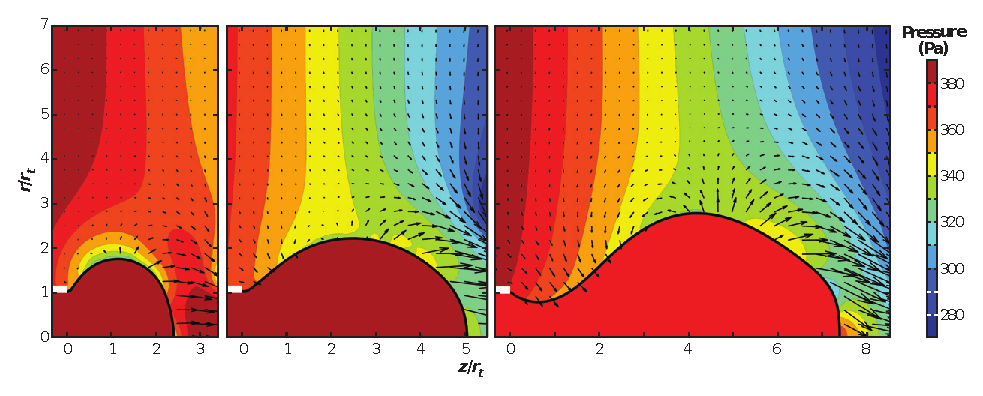
\includegraphics[width=\linewidth]{introduccion/figuras/esquemaBurbuja.eps}
\caption{Contornos de presión en las fases iniciales del proceso de formación de una burbuja para un número de Bond, $Bo = 0.245$. Cortesía de~\cite{Rodriguez-Rodriguez2015b}}
\LABFIG{esquemaBurbuja}
\end{figure}

Sintetizando una vez más las ideas expuestas en~\cite{Rodriguez-Rodriguez2015b}, el proceso de formación de una burbuja en una piscina en reposo puede esquematizarse en las siguientes etapas:

\begin{itemize}
\item En primer lugar, para satisfacer \EQ{continuidad}, el volumen de la burbuja debe aumentar, lo que provoca velocidades radiales en el líquido hacia fuera de la burbuja. 
\item La presión del gas en el interior de la burbuja es prácticamente uniforme, y debe adaptarse a la del líquido exterior en algún punto entre $z = 0$ (véase la \FIG{esquemaBurbuja}) y $z = 2R_{b}$, el cenit de la misma, supóngase en $z \sim R_{b}$. 
\item A medida que el radio de la burbuja aumenta, la punta de la burbuja se encuentra con una sobrepresión respecto al líquido exterior del orden de $\sim \rho g R_{b}$, lo que contribuye a que el gas acelere al líquido exterior, mientras que, en $z = 0$, es el líquido el que ejerce una sobrepresión sobre la base de la burbuja del orden de $\sim -\rho g R_{b}$, lo que conlleva que el líquido induzca velocidades hacia el interior de la burbuja. 
\end{itemize}

Por lo tanto, si nos ceñimos al caso no viscoso, la burbuja se desprenderá del inyector cuando la velocidad hacia adentro en $z = 0$, que surge del balance de \EQ{rayleighPlesset}, $\Delta p = p_{exit} - 2\sigma/R_{b} \sim \rho \dot{R}_{b}$ coincida con la velocidad hacia afuera impuesta por continuidad, $\sim Q_{g}/\left(4\pi R_{b}^{2}\right)$.

\begin{equation}\LABEQ{dbestimado}
\dfrac{Q_{g}}{R_{b}^{2}} \sim 	\sqrt{\dfrac{\Delta p}{\rho}} \sim \sqrt{g R_{b}} \Rightarrow d_{b} \sim \left(\dfrac{Q_{g}}{g^{1/2}}\right)^{2/5}
\end{equation}

siendo, finalmente, la frecuencia de producción 

\begin{equation}\LABEQ{fbestimado}
f_{b}\sim \dfrac{Q_{g}}{d_{b}^{3}} \sim	\left(\dfrac{g^{3}}{Q_{g}}\right)^{1/5}
\end{equation}

Así, aunque puede emplearse este sencillo método para producir burbujas simplemente inyectando gas en el seno de un líquido en reposo, la burbujas obtenidas poseen un diámetro significativamente mayor que el radio del inyector y con frecuencias que decrecen con el caudal, por lo que no resulta un método adecuado para satisfacer las demandas que las aplicaciones actuales requieren en lo que a diámetros y frecuencias se refiere\cite{Rodriguez-Rodriguez2015b}. Ello ha propiciado el desarrollo de tecnologías más sofisticadas basadas en dispositivos microfluídicos los cuales, en esencia, buscan aumentar el gradiente de presión (esto es, la gravedad efectiva) al que se ve sometida la gota en su proceso de generación. 




\section{Dispositivos para la generación de microburbujas}\LABSEC{tecnologias}


Una vez que se han descrito las ecuaciones necesarias para la compresión de los fundamentos de la generación de burbujas en el seno de un líquido, se está en disposición de enumerar y describir de forma sucinta las tecnologías más relevantes que, actualmente, se emplean para producir masivamente las mencionadas burbujas. Conviene recordar que las soluciones tecnológicas que aquí se presentan no son las únicas que permiten la producción de burbujas con tamaños submilimétricos; en efecto, en aplicaciones industriales como los reactores químicos, los esfuerzos de cortadura fruto de la turbulencia son los responsables de que la formación de burbujas que, aunque micrométricas y a grandes frecuencias, son generadas con un alto PDI~\cite{Rodriguez-Rodriguez2015b}.

De nuevo, al igual que se realizó en \SEC{fundamentos}, se respetará la estructura de~\cite{Rodriguez-Rodriguez2015b} para presentar las tecnologías que a continuación se describen, no extendiénsose en exceso y pudiendo encontrar el lector una descripción más detallada tanto en el \textit{review} como en las referencias citadas en él. Así pues, en la \FIG{tecnologias}, se describen de forma esquemática los dispositivos más relevantes para la producción de burbujas actualmente. En la figura se pueden distinguir dos tipos principales de tecnologías: aquellas emplean una corriente de líquido para provocar el colapso de la corriente gaseosa para la formación de burbujas (\FIG{tecnologias}a-d) y aquellas que en las que se emplean ultrasonidos (\FIG{tecnologias}e-f). A su vez, de entre las primeras, se puede distinguir en aquellas en las que el líquido es inyectado en la misma dirección que la corriente gaseosa (\FIG{tecnologias}a-c) y aquellas en las que el líquido y el gas se encuentran de forma perpendicular (\FIG{tecnologias}d). Finalmente, la diferencia principal entre los dispositivos de \emph{flow-focussing} (\FIG{tecnologias}b-c), y los de \emph{coflow} es que en el primero se hace pasar ambos fluidos a través de un estrechamiento, lo que acelera colapso y permite generar burbujas más pequeñas~\cite{Rodriguez-Rodriguez2015b}. En esta sección, nos centraremos sólo en los 4 primeros, debido a la analogía que los mismos presentan con la solución tecnológica de la que trata este estudio. 


\begin{figure}
\LABFIG{tecnologias}
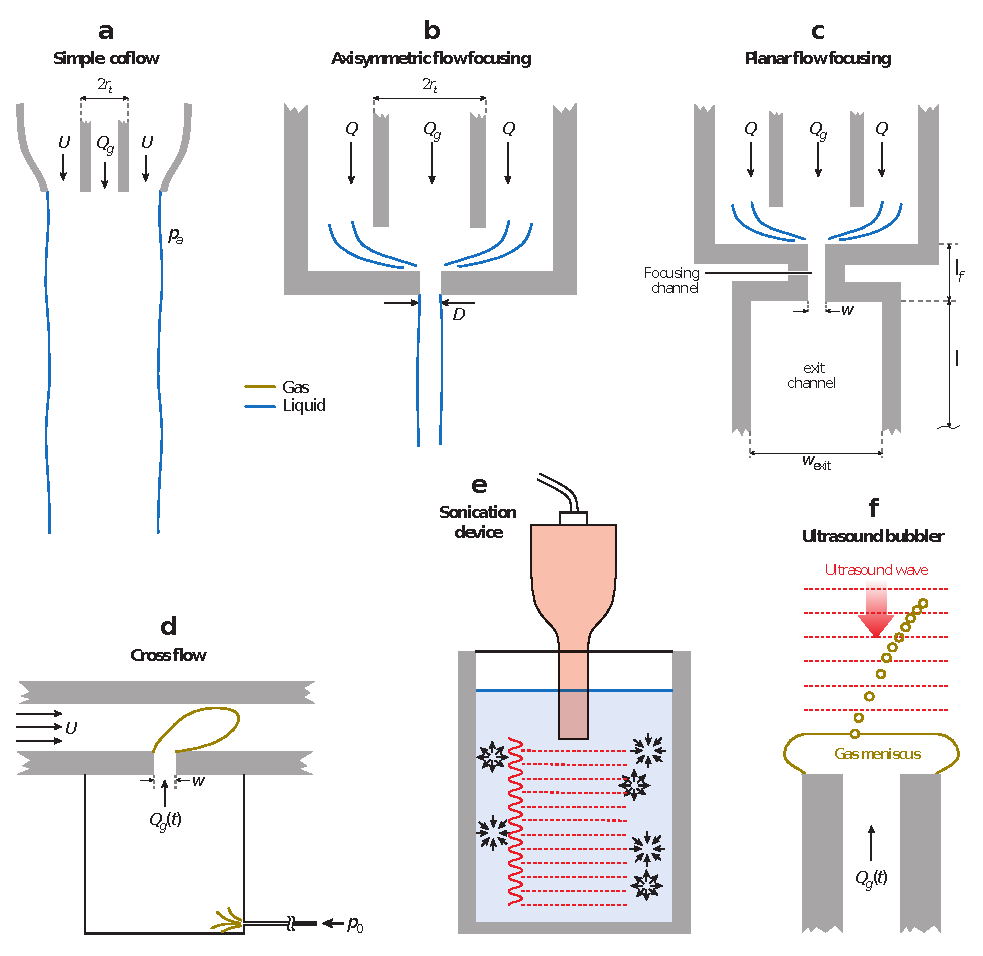
\includegraphics[scale=1]{introduccion/figuras/tecnologias.eps}
\caption{Representación esquemática de los diferentes dispositivos que identiican la tecnología utilizada en la producción de burbujas monodispersas. Figura adaptada de~\cite{Rodriguez-Rodriguez2015b}.}
\LABFIG{tecnologias}
\end{figure}

\subsection{Dispositivos de Coflow}\LABSSEC{coflow}

Un dispositivo de tipo coflow es aquél como el mostrado en la \FIG{tecnologias}a, donde la corriente gaseosa y la de líquido son inyectadas en la misma dirección y de forma libre. Las condiciones en las que usualmente se opera este tipo de dispositivos son aquellas en las que el número de Reynolds y Webber son tales que $Re = \rho U r_{t}/\mu \gg 1$ y $We = \rho U^{2} r_{t}/ \sigma$. Bajo estas condiciones, las frecuencias de producción, $f_{b}$ y los diámetros equivalentes de las burbujas obtenidas, $d_{b} = \left[\left(6Q_{g}\right)/\left(\pi f_{b}\right)\right]^{\left(1/3\right)} $, dependen sólo del ratio de velocidades gas-líquido, $U_{g}/U$, y del ratio $r_{t}/U$. Además, en los casos bajo consideración donde $We \gg 1$, el líquido exterior impone la velocidad a la que la interfase es transportada, con lo que se previene la coalescencia ya que las burbujas son transportadas a la velocidad del líquido~\cite{Sevilla2005a}. Precisamente, en una operación normal con este tipo de dispositivos, la velocidad del gas suele ser mayor que la del líquido, con lo que las burbujas son generadas cerca de la punta del inyector. Siguiendo las mismas ideas que el proceso basado en las fases de expansión y posterior colapso descrito en \SEC{fundamentos}, en \cite{Gordillo2007a} se desarrolla un modelo simple para la fase de colapso en el que puede comprobarse que, en el límite en el que $U_{g}/U \gg 1$, la frecuencia escala como $f_{b}\simeq 0.15U/r_{t}$. 

Por otro lado, el caso contrario en el que $Re \ll 1$ no ha sido muy reportado en la literatura~\cite{Rodriguez-Rodriguez2015b}. En este caso, en lugar del número de Webber, el parámetro adimensional que gobierna el problema es el número capilar, $Ca = \mu U /\sigma$, además del ratio $U_{g}/U$ como en el caso anterior y del ya descrito número de Bond, $Bo$. En este caso, tras el exhaustivo estudio numérico de~\cite{Suryo2006a}, se tiene que el diámetro de las burbujas decrece cuando el ratio $U_{g}/U$ también lo hace. 

\subsection{Dispositivos de Cross-Flow}\LABSSEC{crossflow}

Los dispositivos de tipo Cross-Flow son aquellos como los mostrados en la \FIG{tecnologias}d, donde puede apreciarse que el gas es inyectado de forma perpendicular al líquido a través de una junta en T. Para tener buen control y repetibilidad en los tamaños de las burbujas, estos dispositivos operan a números de Reynolds muy bajos, por lo que su mayor campo de amplicación se encuentra dentro de la microfluídica. Dado que operan a $Re \ll 1$, se observan diferentes regímenes en función del número capilar, $Ca$, como son el \emph{squeezing, dripping} o \emph{jetting}. De entre ellos, el que parece más apropiado para el control del diámetro de las burbujas es el \emph{squeezing}, lo que ocurre cuando $Ca \lesssim \\mathcal{O}\left(10^{-2}\right)$. Por otro lado, una de las principales desventajas del empleo de este tipo de dispositivo es la baja frecuencia de producción derivada de la operación a bajos números capilares. En efecto, si se pretende aumentar la velocidad del líquido para aumentar dicha frecuencia, también se producirá un aumento del numero capilar, lo que limita en general la frecuencia de producción de estos dispositivos a $f_{b}\sim 10^{3} \mathrm{Hz}$. 

Tanto los dispositivos con configuraciones de tipo Cross.Flow como los de Coflow permiten tener control de forma separada del diámetro de las burbujas y de su frecuencia, variando $Q_{g}$ y $Q$. Sin embargo, a pesar de ser dispositivos microfluídicos de tamaños del orden de las centenas de milímetros (o mayores), su geometría limita el tamaño mínimo de las burbujas que se pueden obtener. Esta dificultad puede ser superada e través de otro método conocido como \emph{Flow-Focussing} que utiliza una geometría un tanto diferente como se verá en la próxima subsección. 

\subsection{Dispositivos de Flow-Focussing}\LABSSEC{flowfocussing}


La sencillez de los dispositivos descritos anteriormente posee un notable inconveniente, pues si se elmina la inyección de gas las líneas de líquido son casi paralelas, con lo que los gradientes de presión existentes son prácticamente despreciables~\cite{Rodriguez-Rodriguez2015b}. La demanda de diámetros cada vez menores de las burbujas hace que sea tecnológicamente inviable reducir tanto como se desee el diámetro del inyector, por lo que otras soluciones han emergido para paliar las limitaciones de las configuraciones de coflow y crossflow; una de ellas, es el empleo de dispositivos de \emph{Flow-Focussing}. En geometrías de flow-focussing como las mostradas en la \FIG{tecnologias}b-c, la presencia del estrechamiento provoca (además de un coflujo de líquido y gas que previene la aparición de coalescencia) un gradiente longitudinal de presión, cuyo efecto principal es el de reducir el diámetro final de las burbujas obtenidas. Los primeros en reportar este fenómeno fueron~\cite{Ganan-Calvo2001a}, obteniendo burbujas de tamaños $d_{b} \mathcal{O}\left(10 \mu m\right) < D$, controlando simplemente el ratio $Q_{g}/Q$  y el caudal de líquido exterior $Q = \pi D^{2} U/4$, con $D$ el diámetro del estrechamiento. En efecto, el papel del gradiente axial de presión es análogo al jugado por la gravedad en el caso de la \EQ{dbestimado}, esto es, tomando $\Delta p_{exit} = \nabla p R_{b}$, y teniendo en cuenta que el gradiente de presión puede ser obtenido de forma estimada de las ecuaciones de Navier-Stokes como

\begin{equation}\LABEQ{focusGradPres}
\rho \dfrac{D\mathbf{u}}{Dt} = -\nabla p \Rightarrow \nabla p \sim \rho \mathbf{u} \cdot \nabla \mathbf{u} \sim \rho U^{2}/D
\end{equation}

se tiene, sustituyendo $ \Delta p $ en \eqref{eq:dbestimado},

\begin{equation}\LABEQ{focusDbEstimado}
\dfrac{d_{b}}{D} \sim \left(\dfrac{Q_{g}}{Q}\right)^{2/5}
\end{equation}

siendo pues la frecuencia de burbujeo 

\begin{equation}\LABEQ{focusFb}
f_{b} = \dfrac{6 Q_{g}}{\pi d_{b}^{3}} \propto \dfrac{U}{D}\left(\dfrac{Q_{g}}{Q}\right)^{-1/5}
\end{equation}

por lo que este dispositivo también permite controlar de forma separada tamaño y frecuencia de producción simplemente a través de la variación de los reatios $Q_{g}/Q$ y de la velocidad del líquido $U$. Uno de los principales escollos en el uso de este tipo de dispositivos se encuentra en la dificultad que supone conseguir un buen alineamiento entre los diferentes canales, lo que introdujo la configuración de la \FIG{tecnologias}c, que permite simplificar esta labor.


\subsection{Otros dispositivos y breve reflexión}\LABSSEC{ConclusionDevices}

Existe, además de los descritos en los apartados anteriores, otros dispositivos para generar burubujas de tamaño micrométrico de forma monodispersa, como son aquellos basados en la aplicación de ondas acústicas, tal y como se muestra en la \FIG{tecnologias}e-f, y lo que es más, nada impediría (en principio) combinar estos dispositivos con los anteriores, si se pretende reducir aún ás el diámetro de las burbujas~\cite{Rodriguez-Rodriguez2015b}. A través de los ejemplos más significativos de dispositivos que aquí se han presentado, el lector puede estimar que el tamaño característico de estos dispositivos se encontrará en un rango comprendido entre $\sim \mathcal{O}(10 \mu\, m)$ hasta  $\sim \mathcal{O}\left(10 \,\mathrm{mm}\right)$, lo que a priori puede suponer una dificultad tanto de fabricación como de operación; además, a la dificultad de manejo de los instrumentos microfluídicos habría que sumar la limitación existente en la frecuencia máxima de producción, que estaría limitada por el tamaño de los dispositivos y cuya solución se encontraría en la fabriación de un número mayor de estos. Cabe entonces preguntarse si los mecanismos físicos ya descritos y que subyacen bajo los diferentes procesos de producción de microburbujas aquí presentados van aparajados necesariamente del empleo de dispositivos microfluídicos. En efecto, si bien a lo largo del capítulo se ha podido comprobar que existe una clara dependencia con el diámetro del inyector del gas (lo que apoya la necesidad del empleo de la microfluídica), también es cierto que las condiciones de contorno que el líquido exterior impone sobre la corriente gaseosa, bien únicamente mediante el transporte a la velocidad del líquido de la interfase (coflow y cross-flow) o bien sumando el gradiente longitudinal de presión provocado por un estrechamiento (flow-focussing), no tendrían (en principio) porqué ir ligadas taxativamente al empleo de geometrías micrométricas.  

Así pues, en la siguiente sección de este capítulo se discute con más detalle el papel que el gradiente de presión juega en la formación de burbujas, prestando especial atención para ello en una técnica conocida como \emph{Confined-Selective-Withdrawal} que presenta características comunes tanto a las configuraciones de coflow y flow-focussing. Se pretende así reforzar la idea de la importancia que juega el gradiente de presión en la formación de burbujas para, finalmente, plantear si cabría la posibilidad de plantearse un dispositivo capaz de generar microburbujas monodispersas de forma masiva con dimensiones características mucho mayores que las de los dispositivos empleados actualmente. 

\section{Influencia del gradiente de presión}\LABSEC{gradPres}

A lo largo de la \SEC{tecnologías}, se ha podido comprobar como el papel del líquido exterior en la generación de microburbujas puede ir desde simplemente imponer la velocidad de la entrefase previniendo la coalescencia hasta ejerecer un efecto análogo al de la gravedad a través del gradiente axial de presión. Las conclusiones extraídas en la \SSEC{ConclusionDevices} motivan indagar un poco más en el papel que dicho gradiente longitudinal de presión puede jugar en el proceso de formación de burbujas, por lo que se van a presentar de forma sucinta los resultados obtenidos~\cite{Evangelio2015b} donde se obtuvieron burbujas de tamaño micrométrico empleando la técnica conocida como \emph{Confined Selective Withdrawal}.

\begin{figure}[hbtp!]
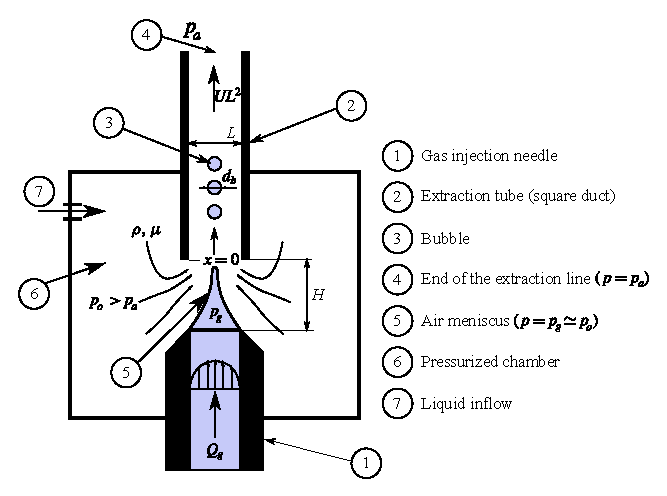
\includegraphics[scale=1]{introduccion/figuras/esquemaCSW.eps}
\caption{Esquema del dispositivo empleado en~\cite{Evangelio2015b} para la producción de microburbujas con la técnica de Confined Selective Withdrawal. Imagen adaptada de~\cite{Evangelio2015b}}
\LABFIG{esquemaCSW}
\end{figure}

 En la \FIG{esquemaCSW} se describe esquemáticamente el funcionamiento de este dispositivo. El dispositivo consiste en cámara presurizada a $p_{0}$ con un líquido, de densidad $\rho$ y de viscosidad $\mu$, que se suministra desde el exterior y que descarga a $p_{a} < p_{0}$ a través de una salida a través de un capilar (en este caso de sección cuadrada) de dimensiones características $L = 1\,\mathrm{mm}$. El capilar se encuentra perfectamente alineado con una aguja donde se inyecta el gas con caudal $Q_{g}$ y que se encuentra a una distancia $H$ del capilar. Como puede observarse en la \FIG{fenomenologia}, para velocidades del líquido en el capilar inferiores a una $U < U^{*}$, el menisco emite burbujas de forma pulsante y de diferentes diámetros~\cite{Evangelio2015b}. Sin embargo, por encima de esta velocidad, se puede observar que el menisco de aire se mantiene estable para una regíon $x \leq x_{s}$, lo que propicia la aparición de un régimen de producción de burbujas monodispersas; la condición de equilibrio de la que resulta $x_{s}$ será discutida más adelante. Finalmente, en la \FIG{produccionEstable} se muestra como, para valores de $U > U^{*}$, aguas abajo de la zona estacionaria ($x \leq x_{s}$), se produce un cilindro de gas de diámetro $d_{g}$ y longitud $\ell$ que, finalmente, culmina con la producción de una nueva burbuja; una vez la burbuja es emitida y transportada a la velocidad del líquido, se inicia nuevamente el proceso de formación de otra burbuja a través del mecanismo descrito. 
 
\begin{figure}[hbtp!]
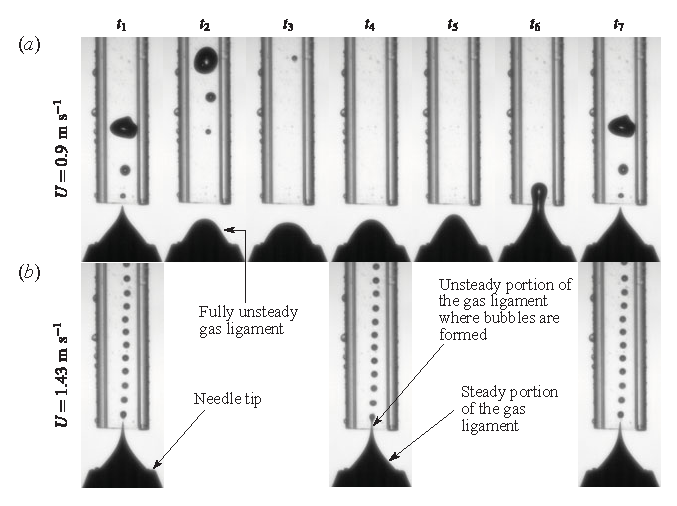
\includegraphics[scale=1]{introduccion/figuras/fenomenologia.eps}
\caption{Diferentes regímenes de burbujeo en función de la velocidad $U$ a la que el líquido circula a través del capilar. En (a) se visualiza el caso en que $U < U^{*}$, por lo que no se tiene un régimen de burbujeo constante, mientras que en (b), $U > U^{*}$, se consigue alcanzar un régimen de producción de burbujas monodispersas. Imágenes adaptadas de~\cite{Evangelio2015b}.}
\LABFIG{fenomenologia}
\end{figure}

Aunque en~\cite{Evangelio2015b} se analiza tanto el caso viscoso como el no viscoso, en esta sección nos centraremos únicamente en los casos $Re \gg 1$, ya que será el caso de interés para el dispositivo que aquí se describe. Antes de comenzar el análisis, conviene notar que la presión del gas, $p_{g}$, que además se considera constante a lo largo del mismo según la hipótesis ya comentada en la \SEC{fundamentos}, debe de encontrarse en equilibrio con la del líquido a la salida de la aguja, donde la velocidad del líquido es casi nula, por lo que puede suponerse que $p_{g} \simeq p_{0}$. Así, para obtener un menisco de aire estable en la región $x \leq x_{s}$, la diferencia de presiones $p_{0} - p\left(x\right)$ debe estar en equilibrio con la presión capilar. En efecto, considerando que el hilo gaseoso tenga un diámetro $d_{g}$, llamando $U_{0}$ a la velocidad en el centro del tubo capilar, y teniendo en cuenta el cumplimiento de la ecuación de continuidad

\begin{equation}
Q_{g} = \dfrac{\pi d_{g}^{2}}{4}U_{0} \Rightarrow d_{g} \sim \left(\dfrac{Q_{g}}{U_{0}}\right)^{1/2}
\LABEQ{continuidadLigamento}, 
\end{equation}

se tiene que 

\begin{equation}
p_{0} - p\left(x_{s}\right) = \dfrac{2\sigma}{d_{g}} \simeq \dfrac{2\sigma}{\left(Q_{g}/U_{0}\right)^{1/2}}
\LABEQ{equilibrioLigamento}
\end{equation}

lo que proporciona la condición de equilibrio para que exista un menisco de aire estacionario en $x \leq x_{s}$. Tanto en \eqref{eq:contiuidadLigamento} como en \eqref{equilibrioLigamento}, la expresión de $U_{0}$ vendrá determinada por el tipo de flujo que exista en el capilar, lo que para el caso en el que $Re \gg 1$ y teniendo en cuenta los resultados de las simulaciones
\footnote{En~\cite{Evangelio2015b} se realiza una simulación del dominio considerando este como axilsimétrico y sin simular la fase gaseosa, lo que suele realizarse generalmente cuando se desea estudiar la estabilidad de chorros, descomponiendo el campo de presiones como suma de la solución básica más una perturbación (véase como ejemplo~\cite{Gordillo2014a}. En~\cite{Evangelio2015b}, sin embargo, se realiza la hipótesis, verificada \textit{a posteriori}, de que la presencia de las burbujas no perturba el campo de presiones del líquido.} realizadas en~\cite{Evangelio2015b} constituye un perfil uniforme de velocidad; efectivamente, este hecho queda representado por el valor del coeficiente de presión adimensional $\xi = \left(p_{0} - p\left(x\right)\right)/\left(1/2 \rho U^{2}\right) \simeq 1$ en $x = 0$. Así, dado que $p_{0} - p\left(x_{s}\right) \sim 1/2\rho U^{2}$ para $Re \gg 1$ y teniendo en cuenta que la formación de burbujas tnedrá lugar si $p_{0}-p\left(x\right) > \dfrac{2\sigma}{d_{g}}$, la formación de burbujas monodispersas será posible si 

\begin{equation}
\beta = \dfrac{\rho U^{2} L}{4\sigma}q^{1/2} \gtrsim 1 \qquad \mathrm{con} q = \dfrac{Q_{g}}{UL^{2}}
\LABEQ{beta}
\end{equation}

donde $\beta$ en la \EQ{beta} constituye un parámetro similar al número de Webber, $We = \rho U^{2}L^{2}/\sigma$; la validez de \eqref{eq:beta} queda mostrada en~\cite{Evangelio2015b}.

\begin{figure}[hbtp!]
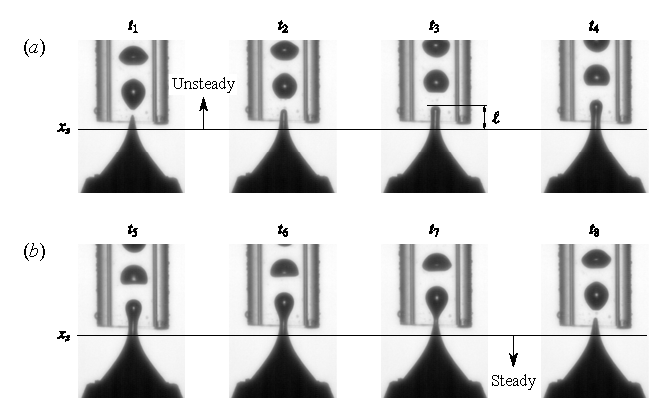
\includegraphics[scale=1]{introduccion/figuras/produccionEstable.eps}
\caption{Secuencia de producción de burbujas a partir de un menisco de aire estable para la región $x \leq x_{s}$. Como se aprecia en la figura, aguas abajo de $x_{s}$, se emite un cilindro de gas de diámetro $\sim d_{g}$ que se extiende una longitud $\ell$. Imagen tomada de~\cite{Evangelio2015b}.}
\LABFIG{produccionEstable}
\end{figure}


Una vez se han descrito las condiciones neesarias para la producción monodispersa de burbujas y se conocen las condiciones de equilibrio estacionario del menisco de aire, se está en condición de describir el resto del proceso de formación, así como las expresiones de los diámetros y frecuencias de producción de las burbujas obtenidas. Una vez que las burbujas se desprenden del ligamento de gas en $Lx \approx Lx_{s} + \ell$, la diferencia de presión $\Delta p = p_{0} - p\left(x\right) -2\sigma/d_{g} > 0$, induce velocidades radiales sobre el ligamento de gas que provoca el inicio del proceso de formación de una nueva burbuja. Dado que durante los instantes posteriores a la eyección de una nueva burbuja el diámetro del cilindro apenas varía, es posible escribir

\begin{equation}
\begin{split}
&\Delta p = p_{0} - p\left(x\right) - 2\sigma/d_{g} = p_{0} - p\left(x_{s}\right) - 2\sigma/d_{g} + p\left(x_{s}\right) - p\left(x\right) \approx \\
& \approx - \dfrac{\mathrm{d}p}{\mathrm{d} x}\left(x_{s}\right)\left(x-x_{s}\right) \approx \dfrac{\mathrm{d}\left(p_{0}-p\right)}{\mathrm{d}x}\left(x_{s}\right)\dfrac{\ell}{L}
\end{split}
\LABEQ{gradPress}
\end{equation}

donde se ha tenido en cuenta la \EQ{equilibrioLigamento} y se ha realizado un desarrollo en serie de Taylor de primer orden de la presión en torno al punto $x = x_{s}$. De este modo, y tal y como se detalla en~\cite{Evangelio2015b}, la \EQ{gradPress} muestra como el proceso de formación de burbujas está gobernado por el gradiente de presión local en el punto $x = x_{s}$, por lo que, como ya se ha comentado previamente, el gradiente de presión local posee un papel absolutamente análogo al que tiene la gravedad en la formación de una burbuja en una piscina en reposo. Por lo tanto, siguiendo el procedimiento que se siguió en la \SEC{fundamentos}, si se sustituye la \EQ{gradPress}, particularizada para el caso $Re \gg 1$, en la ecuación de Rayleigh-Plesset (\EQ{rayleighPlesset}), se tendrá que 

\begin{equation}
\rho R_{b}\ddot{R}_{b} \propto \dfrac{\mathrm{d}\left(p_{0} - p\right)}{\mathrm{d}x}\left(x_{s}\right)\dfrac{\ell}{L}\propto \dfrac{\ell}{2L}\rho U^{2} P_{s}
\end{equation}

siendo $P_{s} = \dot{\xi}\left(x_{s}\right)$. La ecuación anterior junto con la ecuación de continuidad~\eqref{eq:continuidad}, reescrita aquí por conveniencia

\begin{equation}
Q_{g} = \dfrac{\pi}{6}d_{b}^{3} f_{b}
\end{equation}

permiten obtener las frecuencias de producción,

\begin{equation}
\rho \dfrac{P_{s}}{2}\dfrac{U^{2}}{L}\ell \propto \rho R_{b} \ddot{R}_{b} \sim \rho d_{b}^{2}f_{b}^{2} \Rightarrow f_{b} \propto \dfrac{U\sqrt{P_{s}/2}}{\sqrt{L d_{b}}}\sqrt{\dfrac{\ell}{d_{b}}}
\LABEQ{freqGradPres}
\end{equation}

y, finalmente, tomando $\ell \propto d_{b}$ empleando la analogía al caso de formación de burbujas en una piscina en reposo~\cite{Evangelio2015b}, la expresión final de la frecuencia y los diámetros de las burbujas. 

\begin{equation}
f_{b} \propto \dfrac{U\sqrt{P_{s}/2}}{\sqrt{L d_{b}}} \quad \mathrm{y} \quad \dfrac{d_{b}}{L} \propto \left(\dfrac{Q_{g}}{U\sqrt{P_{s}/2}L^{2}}\right)^{2/5}
\end{equation}

El proceso seguido para la obtención de las ecuaciones~\eqref{eq:freqGradPres} y \eqref{dbGradPres} es completamente análogo al descrito en la \SEC{fundamentos} con el gradiente de presión local ejerciendo el papel de la gravedad y con la diferencia que $\rho U^{2}/L \gg \rho g $, lo que atendiendo a las ecuaciones de arriba, se traduce en un aumento de la frecuencia y una disminución de los diámetros obtenidos. Este hecho invita a pensar que, si el proceso de formación descrito está controlado por el gradiente de presión local en $x_{s}$, nada impide imaginar dispositivos generadores de burbujas donde los gradientes favorables de presión puedan obtenerse con geometrías tan diversas como diferentes a la descrita en~\cite{Evangelio2015b}.


\section{Analogía Aerodinámica}\LABSEC{aerodynamics}

Al final de La \SEC{gradPres}, basándose en las ideas de~\cite{Evangelio2015b}, se dejó entrever la posibilidad de obtener gradientes favorables de presión similares a los encontrados en dispositivos de Confned Selective Withdrawal o Flow-Focussing pero con otras geometrías completamente diferentes. La motivación en la exploración de otras geometrías es doble: dispositivos con tamaños alejados de la escala de la microfluídica permitirían no sólo una fabricación y operación más sencilla sino también aumentar notablemente las frecuencias de producción de las burbujas. Así, un ejemplo cotidiano de geometrías donde se producen fuertes gradientes favorables de presión lo constituyen los perfiles aerodinámicos empleados como sección transversal en las alas de los aviones. Dado que la única premisa que, \textit{a priori}, debe cumplir una geometría alternativa a las empleadas actualmente sería conseguir gradientes de presión comparables a los creados en los dispositivos microfluídicos, ¿qué impide pensar que se pueda emplear un ala para producir masivamente microburbujas monodispersas?

Conviene antes de seguir, no obstante, esbozar algunas ideas básicas en aerodinámica que permitirán comprender mejor la posibilidad de emplear un ala como dispositivo generador de burbujas. La Aerodinámica es la parte de la Mecánica de Fluidos que se encarga del estudio del movimiento de gases (generalmente aire) alrededor de un cuerpo. Teniendo en cuenta las propiedades del aire (densidad $\rho_{g} \sim \mathcal{O}(1\,\mathrm{kg/m^{3}})$ y viscosidad $\mu \sim \mathcal{O}(10^{-5}\,\mathrm{Pa \cdot s})$ a $T = 20^{\circ}$) y las velocidades características de un cuerpo que se mueve en él (tómese como ejemplo un coche circulando a $V = 30\,\mathrm{m/s} $ o el ala de un avión a $V = 100\, \mathrm{m/s}$) se tiene que los números de Reynolds característicos del flujo de aire alrededor de un objeto con dimensiones características $L = 1\,\mathrm{m}$ serán $Re = \rho V L / \mu  \sim \mathcal{O}\left(10^{6}\right)$. Bajo estas condiciones los efectos viscosos pueden ser despreciados en la mayor parte del dominio del problema salvo en una delgada región adyacente a la superficie del cuerpo (capa límite), donde la viscosidad impone la condición de contorno de velocidad relativa nula para el fluido con respecto al sólido y donde, por lo tanto, los efectos de inercia y los viscosos son del mismo orden ($Re \approx 1$); el espesor de esta capa puede ser estimado como $\delta_{L} \sim L Re^{-1/2}$, por lo que para el caso del ala de un avión ($L \sim 1\,\mathrm{m}$) esta capa tiene un espesor de apróximadamente 1\,mm. Sin embargo, la importancia de esta delgada capa en la estabilidad del flujo alrededor del cuerpo es capital, ya que si sus efectos no estuvieran confinados a la mencionada región la hipótesis de viscosidad despreciable en el resto del dominio no sería asumible. En efecto, si la corriente experimenta un gradiente adverso de presión (como el que experimenta un fluido cuando circula a través de un canal que se ensancha o el que pueda existir en una esfera aguas abajo del punto más alto de la misma), las velocidades cerca de la pared del sólido son tan cercanas a cero que puede producirse una recirculación del fluido, lo que provocaría el desprendimiento de la capa límite. Para que esto no se produzca, se puede reducir el gradiente desfavorable de presión extediendo la longitud del cuerpo aguas abajo del punto de mínima presión, lo que para el caso de un sólido en el seno del aire significaría emplear cuerpos fuselados (cuerpos con longitud transversal característica mucho menor que la longitudinal) en lugar de cuerpos romos (como sería por ejemplo una esfera). Además, para que la corriente no se desprenda, el ángulo con el que incide la corriente con respecto a línea media longitudinal del sólido, no debe ser muy elevado, ya que de lo contrario el desprendimiento también tendrá lugar. 

\begin{figure}[hbtp!]
\centering
\subfloat[Campo de presión y geometría]{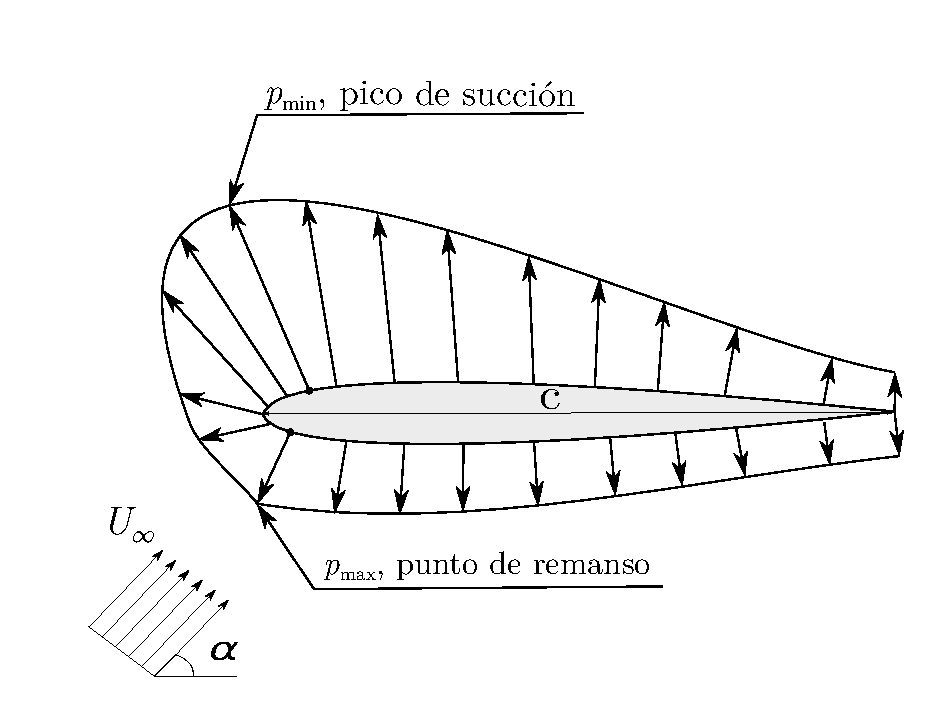
\includegraphics[width=.45\textwidth]{introduccion/figuras/airfoil.eps}\LABFIG{airfoil}}
\subfloat[Líneas de corriente]{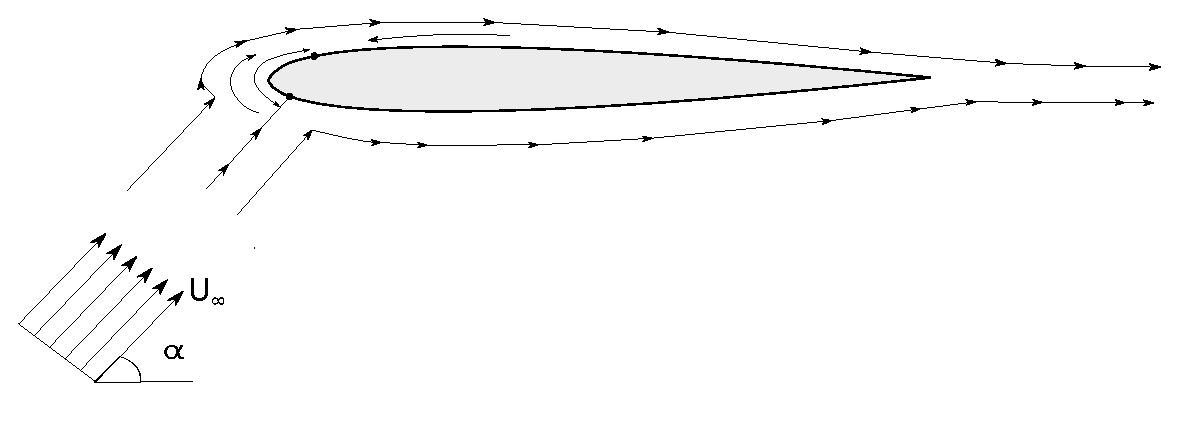
\includegraphics[width=.45\textwidth]{introduccion/figuras/streamlines.eps}\LABFIG{streamlines}}
\caption{Representación esquemática de un perfil aerodinámico que enfrenta una corriente a la velocidad $U_{\infty} $ que forma un ángulo de ataque $\alpha$ con la cuerda, $c$, del perfil. En la \FIG{airfoil} se representan el campo de presión cambiado de signo ($-(p(\mathbf{x})-p_{\infty})$, con $\mathbf{x}\in \Sigma_{s}$, indicando  tanto el pico de succión (punto de mínima presión) como el punto de remanso (punto de máxima presión). En la \FIG{streamlines} se muestra una representación cualitativa de las líneas de corriente alrededor de un perfil aerodinámico. Adicionalmente se representan las zonas de fuertes gradientes favorables de presión, esto es la zona que, conteniendo el borde de ataque, se extiende desde el punto de remanso hasta el pico de succión, y la zona de gradiente desfavorable de presión, que se extiende aguas abajo del pico de succión y que se ha representado con una flecha indicando el sentido de la recirculación que podría producirse en la capa límite.}
\end{figure}

En la \FIG{airfoil} se representa de forma esquemática un perfil aerodinámico que enfrenta una corriente a la velocidad $U_{\infty}$ que forma con la \emph{cuerda del perfil}, $c$, un \emph{ángulo de ataque}, $\alpha$. Considerando que el flujo incidente es uniforme y carente de vorticidad (esto es $\omega = \nabla \times \mathbf{v} = 0$) y despreciando los efectos viscosos en todo el dominio excepto en la capa límite, la velocidad deriva de un potencial, $\mathbf{v} = \nabla \phi$, por lo que, imponiendo la ecuación de continuidad se llega al siguiente problema de contorno

\begin{eqnarray}
\nabla^{2} \phi & = & 0 \\
\nabla \phi \cdot \mathbf{n} & = & 0, \quad \mathbf{x} \in \Sigma_{s}\\
\left|\nabla \phi \right| & \rightarrow & 0, \quad \left|\mathbf{x}\right| \rightarrow \infty
\LABEQ{problemaContorno}
\end{eqnarray}


Con las hipótesis realizadas, la resolución de este problema arroja resultados cualitativos y cuantitativos que ayudarán a comprender mejor el campo de velocidades y en especial de presiones del fluido alrededor del perfil. El problema de la laplaciana, que puede ser resuleto con un método de elementos de cotorno%INCLUIR SI DA TIEMPO UN APÉNDICE CON EL MÉTODO EMPLEADO!!!!!!
, normalmente se descompone como $\phi = \phi_{\infty} + \phi'$, siendo $\phi_{\infty}$ el potencial correspondiente a una corriente infinita a ángulo de ataque $\alpha$ y $\phi^{'}$ el potencial de perturbación causado por la presencia del perfil. En la \FIG{resultadoPotencial} se muestran los resultados de una simulación realizada con el método de los elementos de contorno para problemas bidimensionales aplicada a un perfil simétrico NACA~0012 que se mueve en el seno de un fluido a un ángulo de ataque $\alpha = 4^{\circ}$. Como se puede observar en la \FIG{upotencial} y más detalladamente en la \FIG{upotencialZoom}, la velocidad longitudinal de perturbación posee un mínimo que se corresponde con el punto de remanso (punto de máxima presión) en la \FIG{cp}; nótese que, por conveniencia, se representa el \emph{coeficiente de presión}, $C_{p} = \left(p-p_{\infty}\right)/\left(1/2\rho U_{\infty}^{2}\right)$, cambiado de signo. Del mismo modo, el máximo de $u'$ se corresponde con el punto de mínima presión (pico de succión) como se muestra en la \FIG{cp} y más detalladamente en la \FIG{cpZoom}. 


\begin{figure}
\centering
\subfloat[Velocidad de perturbación adimensional $u'/U_{\infty}$]{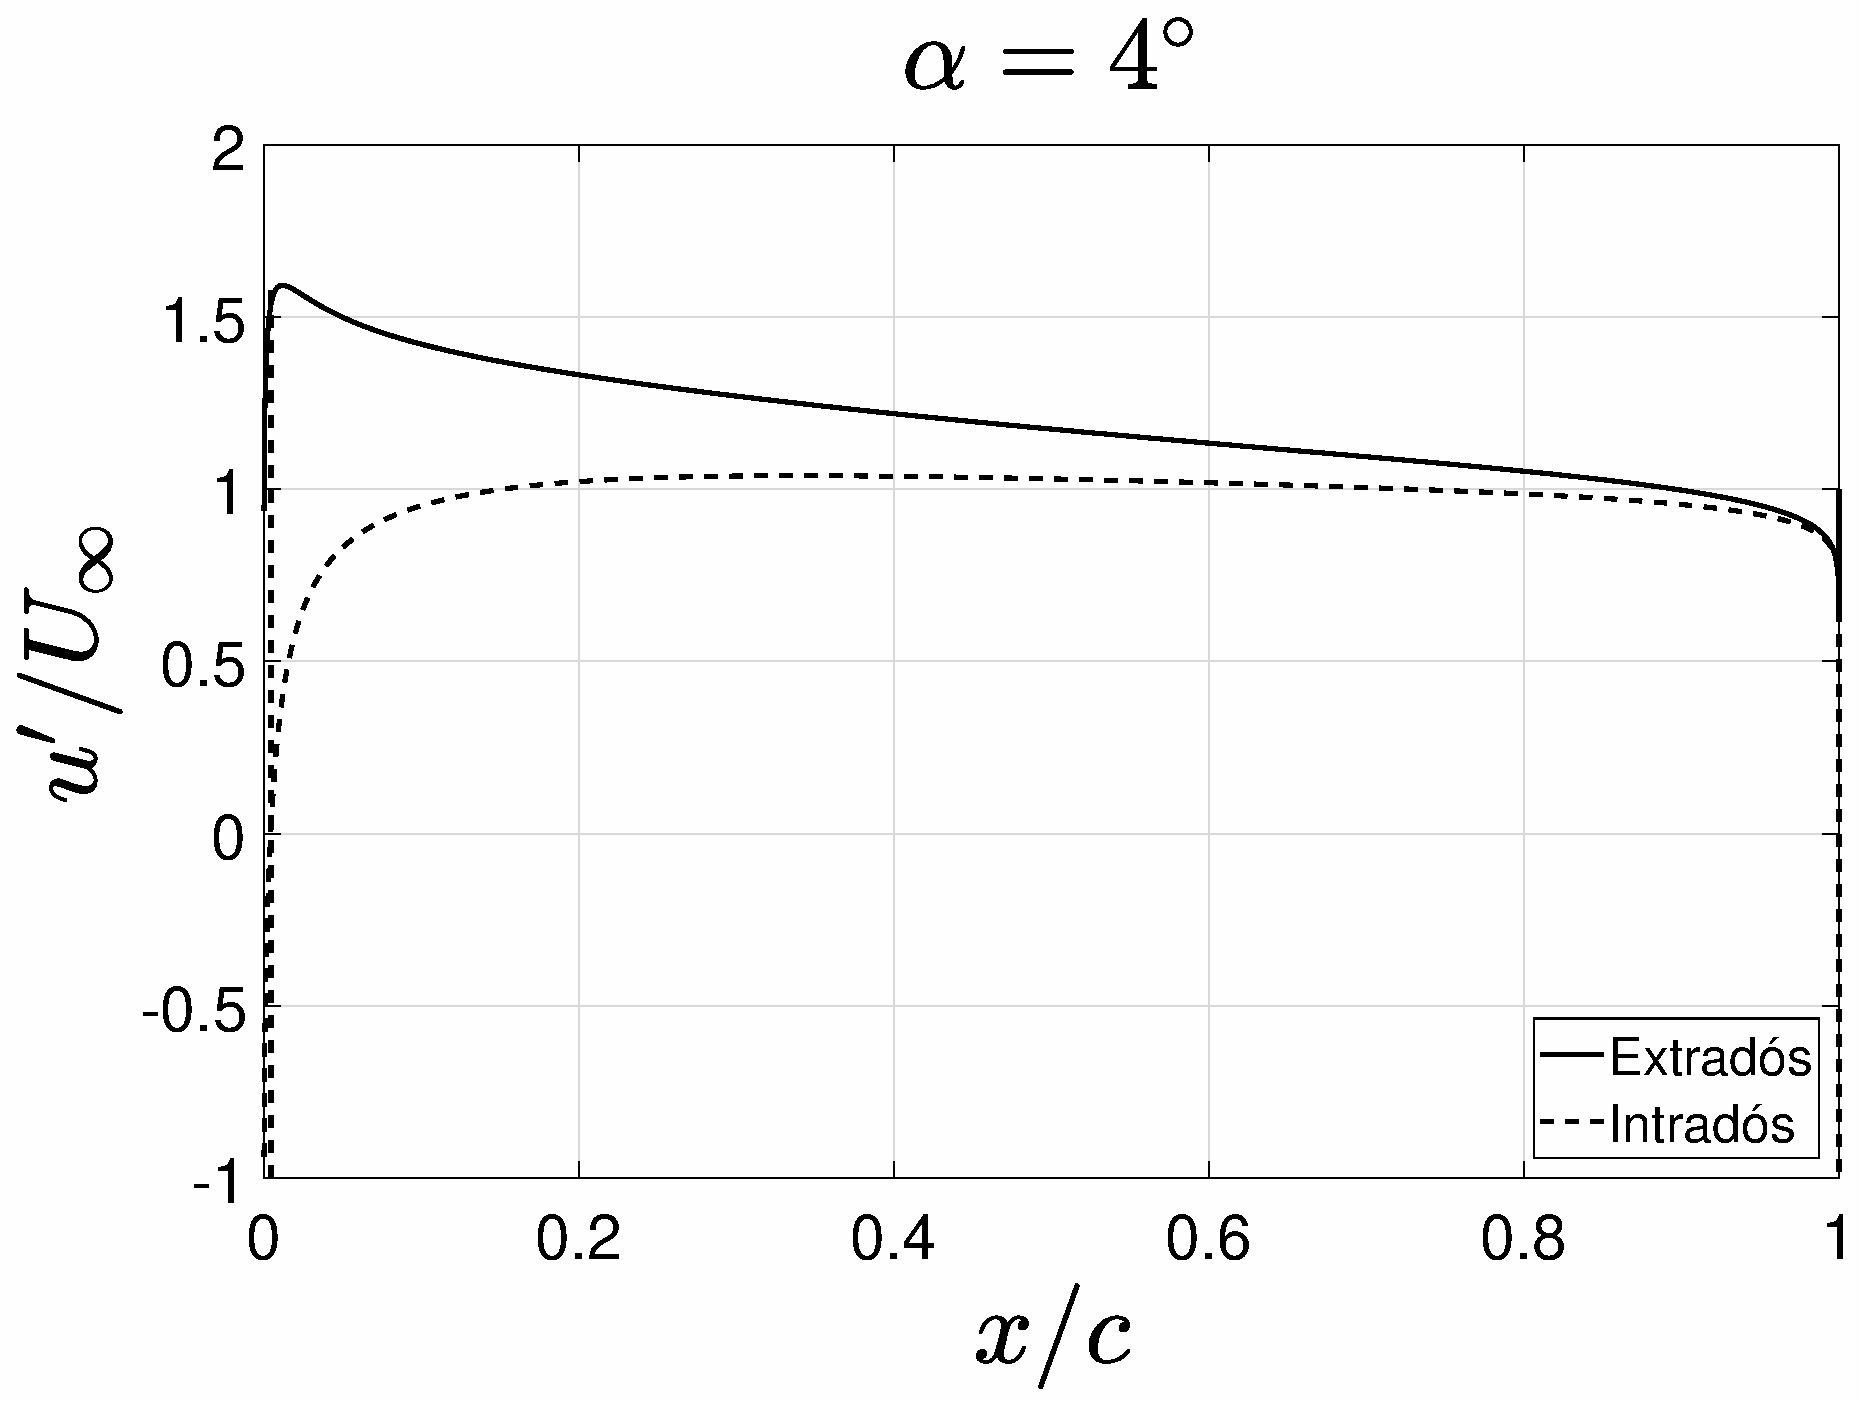
\includegraphics[width = .45\textwidth]{upotencial.eps}\LABFIG{upotencial}}
\subfloat[Zoom de $u'/U_{\infty}$ en el borde de ataque]{\includegraphics[width = .45\textwidth]{uptonecialZoom.eps}\LABFIG{upotencialZoom}} \\
\subfloat[Representación de $-C_{p} = -\left(p-p_{\infty}\right)/\left(1/2\rho U_{\infty}^{2}\right)$]{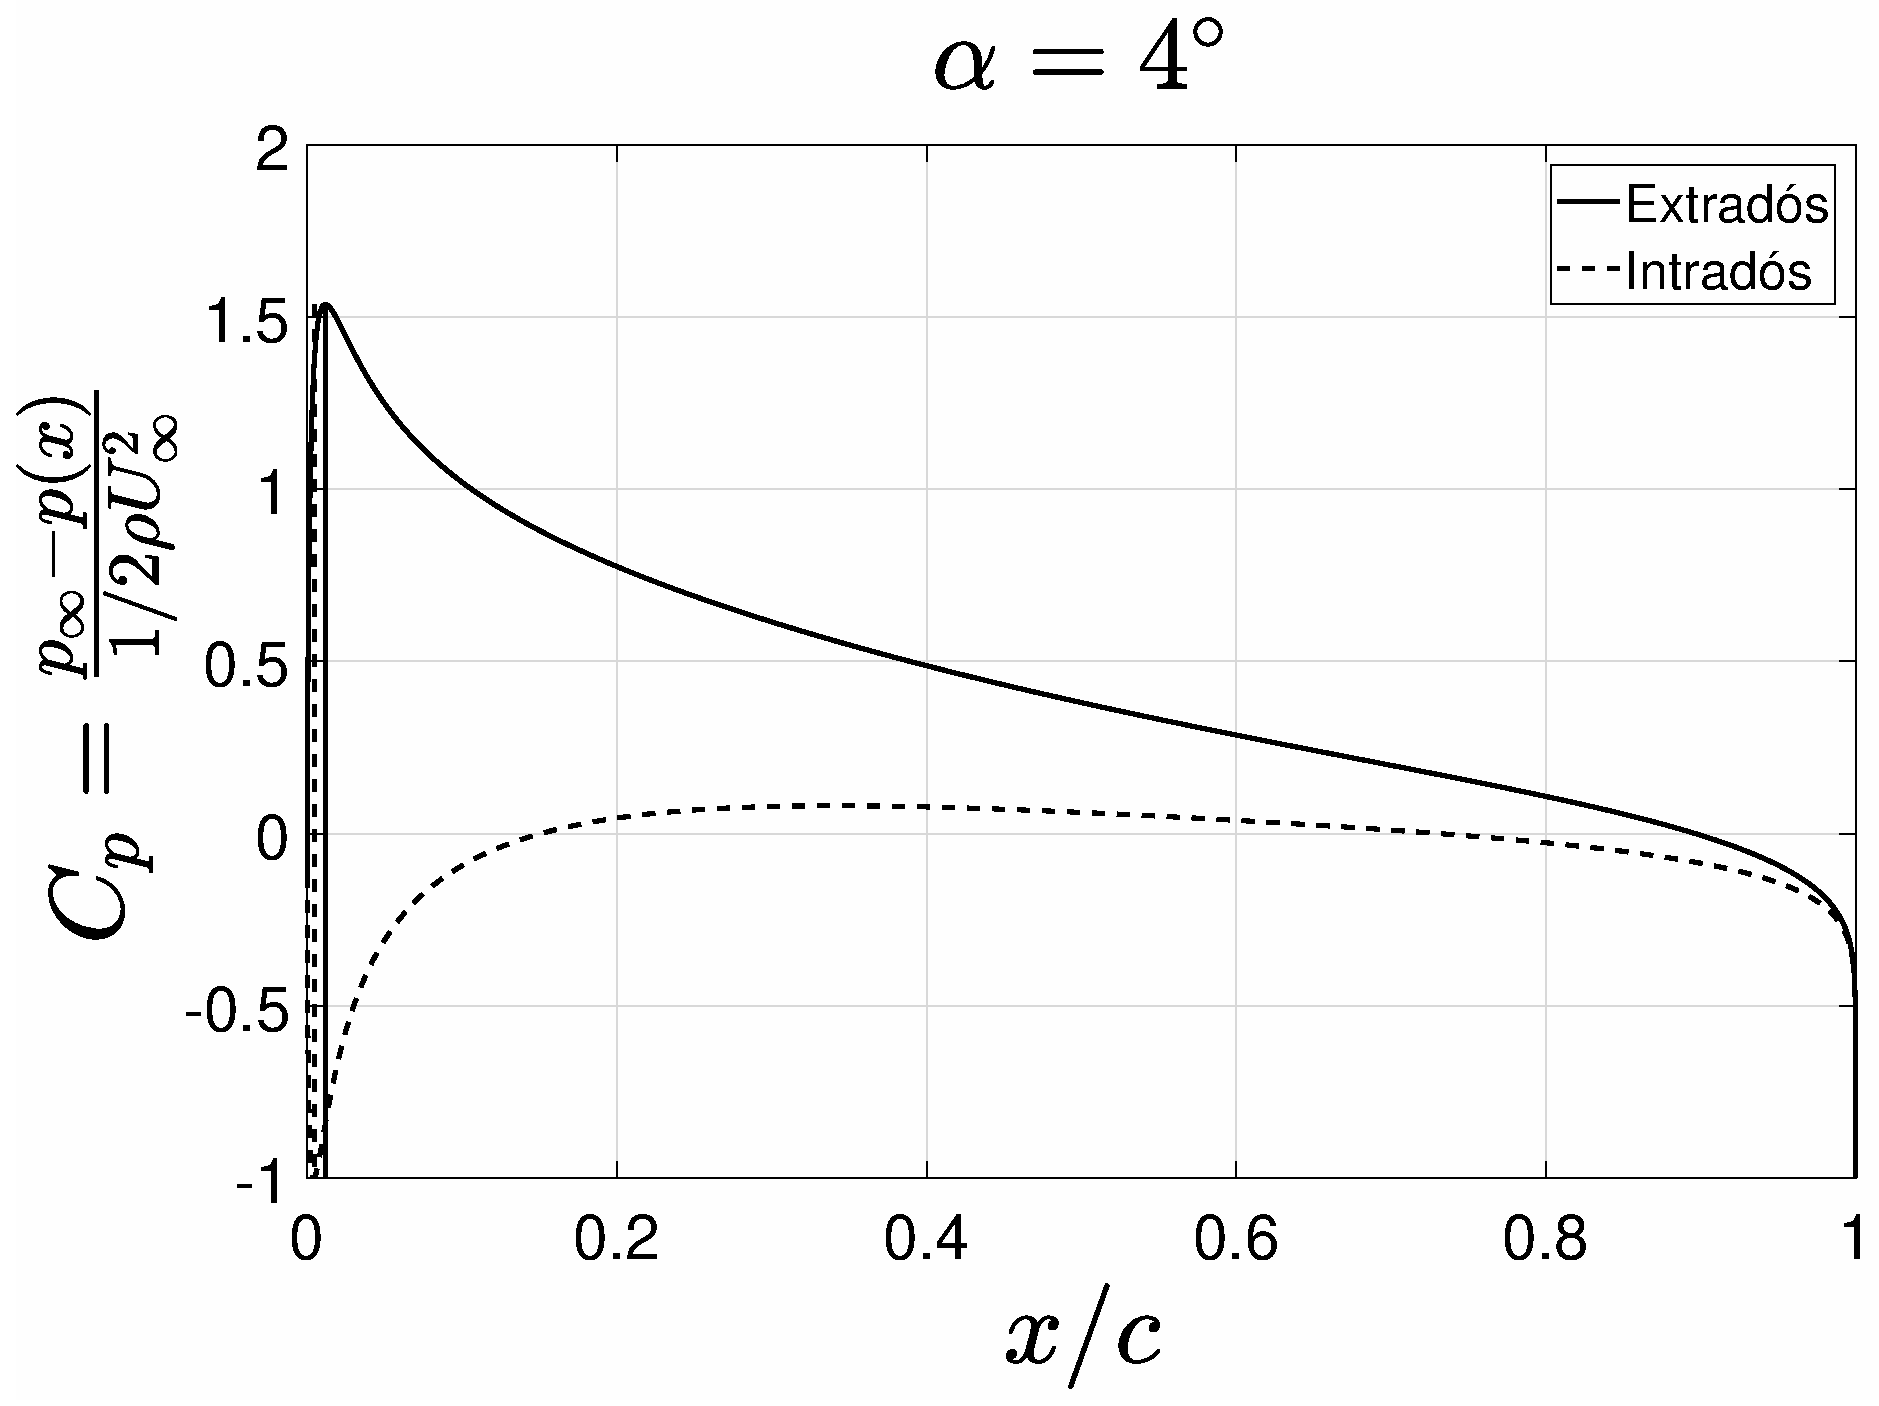
\includegraphics[width = .45\textwidth]{cp.eps}\LABFIG{cp}}
\subfloat[Zoom de $-C_{p}$ en el borde de ataque]{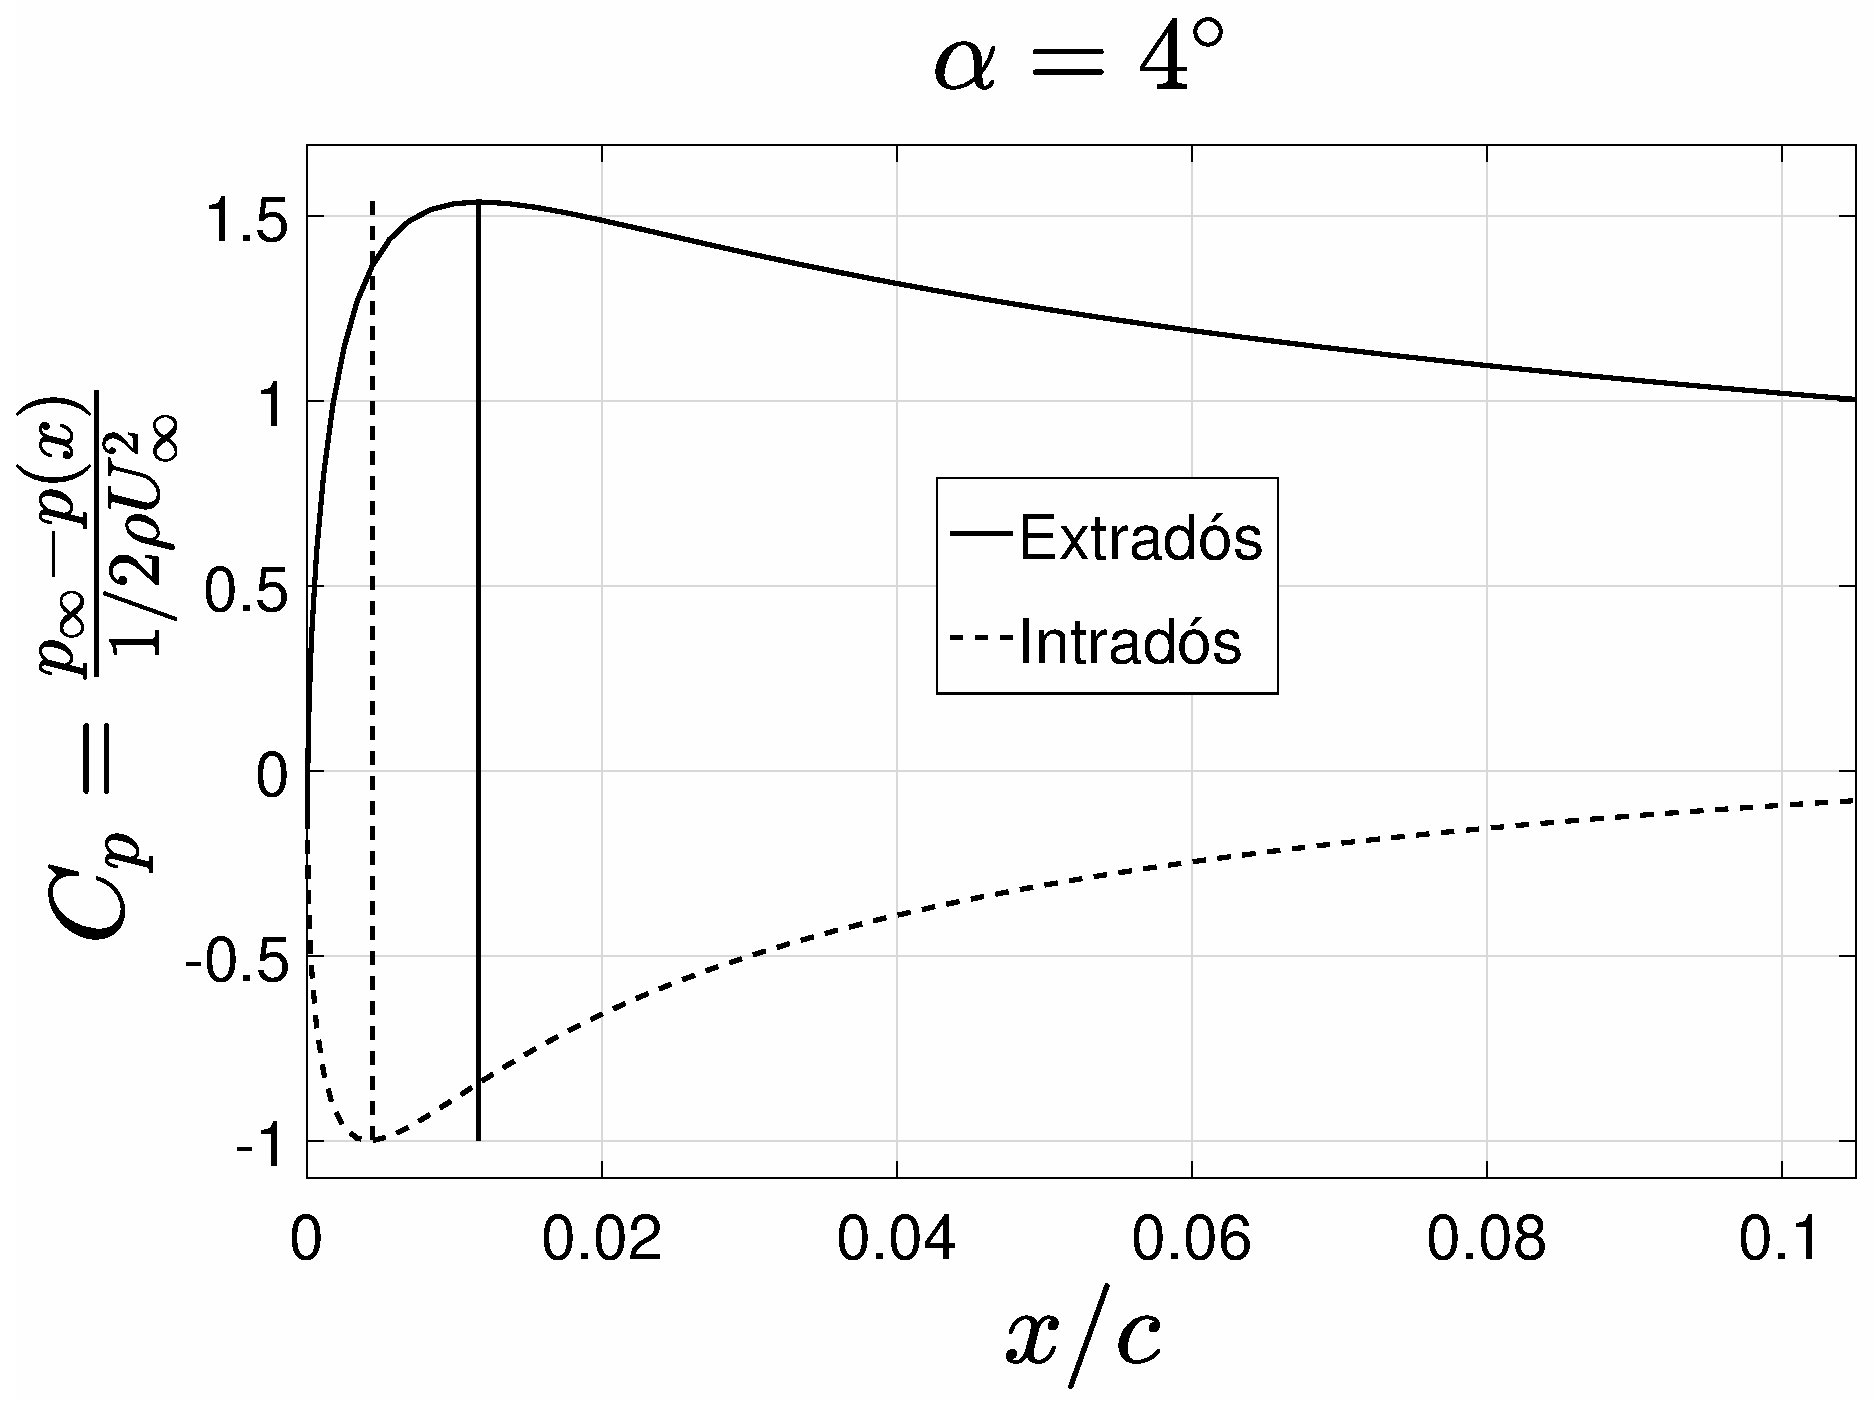
\includegraphics[width=.45\textwidth]{cpZoom.eps}\LABFIG{cpZoom}}
\caption{Resultados de una simulación por el método de elementos de contorno de un perfil simétrico NACA~0012 cuando sobre él incide una corriente con ángulo de ataque $\alpha = 4^{\circ}$. En la \FIG{upotencial} se representa el campo de velocidad longitudinal de perturbación y en la \FIG{cp} su correspondiente campo de presión. La \FIG{upotencialZoom} y la \FIG{cpZoom} se muestra ampliada la zona cercana al borde de ataque, donde existen como puede apreciarse fuertes gradientes favorables de presión.}
\LABFIG{resultadoPotencial}
\end{figure}
%
% Capítulo 2: Ala2D
%
% !TEX root =../pfcTipoETSI.tex
\chapter{Ala acuática bidimensional}\LABCHAP{ala2D}
\pagestyle{esitscCD}
\epigraph{ }{}

%\lettrine[lraise=0.7, lines=1, loversize=-0.25]{E}{l} 
\lettrine[lraise=-0.1, lines=2, loversize=0.25]{A}l final del capítulo anterior se expuso la posibilidad de emplear los gradientes favorables de presión se producen en el borde de ataque de un perfil aerodinámico (cuando sobre el incide una corriente con un ángulo de ataque $\alpha$ determinado) como mecanismo para la formación de microburbujas monodispersas, basándose por analogía en los resultados de~\cite{Evangelio2015b}. El objetivo de este capítulo es pues materializar esta idea diseñando, fabricando y realizando experimentos con un dispositivo generador masivo de microburbujas consistente en un perfil aerodinámico. De este modo, se pretende no sólo demostrar que la producción de burbujas de tamaños milimétricos y submilimétricos no lleva necesariamente aparejado el empleo de dispositivos microfluídicos. Además, se contrastarán las hipótesis realizadas en el capítulo anterior y se explorarán las diferentes dificultades que puedan presentarse en el proceso de escalado. 

La estructura que tomará el capítulo será la siguiente: 
\begin{enumerate}
\item En la \SEC{dessign}, se describe todo lo concerniente al diseño y fabricación del modelo completo, que comprende el dispositivo generador de microburbujas y el montaje experimental del mismo. 
\item En la \SEC{experimentos2D}, se especifican los métodos de experimentación y análisis que serán empleados en la obtención de resultados. De este modo, se describirá la configuración final del \textit{set-up}, el protocolo de experimentación, los datos en bruto obtenidos y el posterior tratamiento para el análisis de los mismos.
\item Finalmente, en  la \SEC{results2D}, se muestran y comentan los resultados obtenidos, realizando las conclusiones pertinentes al final del capítulo
\end{enumerate}

\section{Diseño y fabricación}\LABSEC{dessign}

El objetivo de esta sección es describir de forma detallada los parámetros que configuran el diseño del modelo, tanto aquellos que se refieren al dispositivo en sí como al montaje experimental. Para ello, se describen sucintamente en primer lugar los equipos de los que se dispone y las distintas limitaciones de cada uno de ellos, con el fin de poder acotar el diseño final.

\subsection{Equipos disponibles y limitaciones}\LABSSEC{equipos}



%



%%%%%%%%%%%FIN


\captionsetup[figure]{textformat=period}
\endinput


%
% Capítulo 3: Ala3D
%
% !TEX root =../pfcTipoETSI.tex
\chapter{Ala acuática rotativa}\LABCHAP{ala3D}
\pagestyle{esitscCD}
\epigraph{ }{}

%\lettrine[lraise=0.7, lines=1, loversize=-0.25]{E}{l} 
\lettrine[lraise=-0.1, lines=2, loversize=0.25]{E}{n} el capítulo anterior se demostró como es posible extrapolar los resultados obtenidos en~\cite{Evangelio2015} en un dispositivo microfluídico sin más que reproducir las condiciones en lo que al gradiente favorable de presión se refiere. De hecho, el prototipo de dispositivo generador masivo de microburbujas mostró tener un comportamiento completamente análogo en lo que a los diámetros y frecuencias de producción se refiere, deduciéndose leyes de escala prácticamente idénticas en ambos casos (véase la \SEC{resultados2D}). Sin embargo, pese a haber diseñado un dispositivo capaz de generar microburbujas de forma monodispersa de la misma forma que con la técnica de \textit{confined selective withdrawal}, la implementación de un dispositivo bidimensional para las aplicaciones  tecnológicas reales de hoy en día  resulta tan compleja como insuficiente. Por este motivo, en este último capítulo, nos hemos propuesto ir más allá, no sólo escalando los resultados de un perfil bidimensional al caso de un ala tridimensional de envergadura finita, sino incluyéndola dentro de un nuevo prototipo de dispositivo con un propósito tecnológico concreto. Como ya se mencionó en las primeras páginas del \CHAP{introduccion}, uno de los sectores de la industria que demanda la producción masiva de burbujas de tamaños cada vez más pequeños es el sector de la depuración de aguas, donde una reducción en el diámetro de las burbujas producidas para un caudal de aire determinado aumentaría la eficiencia en la transferencia de oxígeno, o lo que es lo mismo, dados unos requerimientos de suministro de oxígeno (\emph{Oxygen Uptake Rate} - OUR), el caudal total  de aire necesario será menor cuanto menor sean los diámetros de las burbujas producidas, debido al aumento de eficiencia del proceso. Teniendo en cuenta todo lo anterior, el objetivo de este capítulo será el de diseñar, fabricar y testear un prototipo de equipo de agitación y aireación, verificando cómo podrían aplicarse las leyes de escala obtenidas en el \CHAP{ala2D}.

La estructura del capítulo, por lo tanto, seguirá una línea similar a la del capítulo anterior: en primer lugar se describe detalladamente en qué consiste este nuevo diseño de dispositivo, partiendo de los equipos disponibles y diseñando desde cero este nuevo prototipo; acto seguido, se mostrará cómo ha sido la campaña experimental mostrando cuál ha sido el espacio paramétrico explorado en este caso, así como los métodos de postproceso que, aunque similares, amplian los empleados en el caso bidimensional; finalmente, se mostrarán los resultados obtenidos y se tratará de escalar nuevamente el proceso con el fin de poder establecer una clara comparación entre los experimentos microfluídicos en~\cite{Evangelio2015} y los dispositivos aquí presentados.


\section{Diseño y fabriación}\LABSEC{diseno3D}

El objetivo de esta sección es describir cada uno de los componentes que configuran tanto el dispositivo generador de microburbujas como el montaje completo del experimento. Los equipos disponibles para este caso continúan siendo los mismos en lo que a la visualización y suministro de presión se refiere, sin embargo, la tridimensionalidad del problema hace imposible emplear el túnel hidrodinámico como banco de ensayos, por lo que ha sido necesario diseñar y construir un banco apto para esta aplicación. 

\subsection{Esquema general del montaje}\LABSSEC{esquema}

El diseño que aquí se proponga debe satisfacer varias necesidades. En principio, se trata de un equipo rotativo sencillo, consistente en dos palas unidas a un eje que gira accionado por un motor eléctrico. Algunas de las premisas del diseño son las siguientes:
\begin{itemize}
\item Las palas deben encontrarse sumergidas en un tanque de líquido y a la suficiente profundidad como para que el efecto de la entrefase sobre las mismas sea despreciable.
\item   Además debe existir una distancia adecuada a las paredes del tanque con el fin de evitar impactos y velocidades inducidas por el mismo.
\item Por otro lado, las palas deben estar formadas en su sección transversal por perfiles aerodinámicos donde existan fuertes gradientes favoralbes de presión entre el punto de remanso y el pico de succión de cada sección transversal para cada ángulo de ataque.
\item Con el fin de explorar diferentes resultados en función del gradiente de presión, el ángulo de ataque debe poder ser regulable. 
\item Finalmente, se debe conseguir suministrar aire desde el interior de las alas hacia el líquido, lo que deberá hacerse a través del eje de rotación, convirtiéndo al igual que en el caso bidimensional cada pala en un depósito. 
\end{itemize} 

Para cumpliar todas estas premisas, se va a describir el diseño de cada uno de los componentes por separado. 

 
\subsection{Banco de ensayos}\LABSSEC{bancoEnsayos}

El banco de ensayos para un dispositivo de las características mencionadas arriba debe consistir fundamentalmente en un tanque lleno de líquido, en este caso nuevamente agua tanto por su sencillez como por la futura aplicación del propio dispositivo\footnote{Conviene mencionar que el empleo de agua corriente del grifo, a pesar de no ser agua pura, no tiene nada que ver con el tipo de aguas encontrado en la industria de tratamiento de aguas, debido a la abundancia de partículas  y altos contenidos de ácidos como nitratos.}. Por otro lado, el tanque debe realizarse en un material transparente que permita la visualización de las burbujas producidas con el fin de poder medir los diámetros y las frecuencias de producción como se realizó en el \CHAP{ala2D}; se ha optado en este caso por el metacrilato como material de fabriación, debido a su menor coste con respecto al cristal. Aunque  un tanque de geometría cilíndrica sería una solución idónea teniendo en cuenta la axilsimetría del problema, las dificultades y coste que implican la fabriación de un tanque de metacrilato con esta geometría nos llevan a que la mejor solución para esta nueva prueba de concepto es un tanque de metacrilato de sección cuadrada. En cuanto a la altura, se ha considerado suficiente dipsponer de una altura total del tanque de 60~cm, con lo que la altura total de agua estará en torno a los 0.5~m. Con estos requerimientos, y basándose en la experiencia del fabricante, el espesor de pared recomendado no debería ser inferior al mostrado en la \TAB{medidaTanque}, con el fin de aguantar los casi 500~kg del peso del agua. 

\begin{table}
\centering
\begin{tabular}{cccc}
\textbf{Dimensión} & \textbf{Longitud} [m] & \textbf{Altura} [m] & \textbf{Espesor} [mm] \\
\hline \hline
\textbf{Valor} & 1 & 0.6 & 30 \\
\hline
\end{tabular}
\caption{Medidas del tanque empleado en los experimentos del ala acuática rotativa}
\LABTAB{medidaTanque}
\end{table}


Por otro lado, dado que el equipo de visualización empleado será el mismo y una vez más la interfase aire-agua imposibilitaría la visión desde arriba, la grabacion de imágenes a alta velocidad ha de efectuarse desde la zona inferior del tanque, por lo que este debe estar elevado. Para poder realizar los experimentos se requiere por tanto idear una estructura que pueda ser utilizada como banco de ensayos, debiendo la misma dar soporte para la realización de las siguientes tareas:

\begin{itemize}
\item Soporte del tanque a una altura suficiente como para poder incluir el montaje completo del equipo de visualización bajo el mismo. Esta altura debe ser la mínima posible con el fin de evitar aumentar la longitud de los pilares verticales y con ello la inestabilidad por pandeo.
\item Soporte para el equipo rotativo en la zona superior del tanque, el cual debe soportar el peso del motor y sistema de aireación junto con los esfuerzos radiales producidos por el giro del motor. 
\item Estabilidad ante esfuerzos en la dirección perpendicular del eje. En efecto, el movimiento creado por las palas aerodinámicas en el seno del líquido harán que el tanque experimente esfuerzos en su pared que serán, en última instancia, transmitidos a la estructura que constituye el banco de ensayos. 
\end{itemize}

De este modo, teniendo en cuenta todo lo anterior, se ha diseñado y montado una estructura con perfiles de aluminio, que aporta la rigidez y robustez necesarias para satisfacer los requerimientos arriba descritos. En la \FIG{bancoEnsayos} pueden observarse distintas perspectivas de la estructura y el tanque aquí descritos, donde puede observarse que el tanque se sitúa aproximadamente a 1~m de distancia del suelo, dejando espacio suficiente para el montaje del equipo de visualización. Además los dos últimos estantes proveen soporte para el motor eléctrico y el depósito de suministro de presión (este útlimo descrito más adelante), mientras que los perfiles en diagonal aportan la estabilidad suficiente para que, en operación, la estructura no se alabee. 

\begin{figure}
\centering
\subfloat[Perspectiva 1]{\includegraphics[width=.5\textwidth]{bancoEnsayos1.jpg}}
\subfloat[Perspectiva 2]{\includegraphics[width=.5\textwidth]{bancoEnsayos2.jpg}}
\caption{Diferentes perspectivas del banco de ensayos empleado en la campaña experimental. En las figuras se muestra la estructura fabricada a base de perfiles de aluminio junto con el tanque de metacrilato en su interior.}
\LABFIG{bancoEnsayos}
\end{figure}


\subsection{Diseño de las alas}\LABSSEC{disenoAlas3D}

El diseño de las alas empleadas para este dispositivo será muy simiilar al empleado en el dispositivo bidimensional, por lo que muchos de los criterios de diseño seguidos en la \SSEC{disenoAla} pueden ser extrapolados a este caso. Así, por ejemplo, el perfil aerodinámico empleado será el mismo que en el caso bidimensional, es decir el perfil simétrico NACA~0012. Sin embargo, sí que existen una serie de diferencias que merece la pena pararse a detallar. La primera de ellas es que ahora no se dispone de restricciones especiales ni para la cuerda ni para la envergadura del ala, ya que cada una debe ir unida al eje a través de su brazo correspondiente, existiendo por lo tanto un único punto de sujecion situado cerca de la zona de mayor espesor de la sección transversal del ala. En este caso, dado el carácter tridimensional del problema y con la intención de poder aplicar la teoría aerodinámica general para alas esbeltas (descrita en detalle en el Apéndice %PONER AQUIE L APENDICE DE ALAS 
), sería conveniente que su alargamiento, definido como $\Lambda = b^{2}/S$ con $b$ la envergadura y $S$ la superficie en planta, sea tal que $\Lambda > 1$. Para el caso de un ala rectangular sin estrechamiento, la expreisón del alargamiento es simplemente el cociente entre la envergadura y la cuerda, $\Lambda = b/c$, por lo que para el diseño de las palas considerado, una de las restricciones será que $b > c$.

Por otro lado, la sección transversal del ala será muy similar a la del caso bidimensional del \CHAP{ala2D}, ya que el ala actuará como depósito respecto a los orificios de inyección. No obstante, en este caso la inyección de aire se realiza desde un lateral del ala en lugar de hacerla desde la zona del extradós, aprovechando el punto de conexión del ala al eje de rotación a través del brazo. En cuanto a los orificios de inyección, estos consistirán al igual que en el caso del ala bidimensional en idénticos tubos capilares de acero con ratios $D/L_{t} \ll 1$, con el fin de conseguir que la perdida de carga evite variaciones bruscas de caudal por el cambio en la velocidad o el ángulo de ataque incidentes. Una importante diferencia con respecto al caso del perfil bidimensional, es que en este caso no se explorarán diferentes zonas de inyección en torno al borde de ataque, sino que empleando los resultados mostrados en la \SSEC{posicionOrificio}, se ha decidido colocar los puntos de inyección justo en el borde de atque de cada pala. Además, se ha colocado un número mayor de puntos de inyección con la intención de analizar el comportamiento en distintos puntos de la envergadura y de emular aún más el posible de disñeo de un prototipo de dispositivo de aireación y agitación de una planta depuradora. 

\begin{table}
\centering	
\begin{tabular}{c || c c c c c}
\textbf{Elemento} & $\mathbf{b}\,[\mathrm{mm}]$ & $\mathbf{c}\,[\mathrm{mm}]$ & $\mathbf{D}\,[\mathrm{\mu m}]$ & $L_{t}\,[\mathrm{mm}]$ & $\mathbf{g}\,[\mathrm{mm}]$ \\
\hline \hline 
\textbf{Valor} & 200 & 125 & 160 & 30 & 5 \\
\hline

\end{tabular}
\caption{Dimensiones características relevantes del diseño del ala y los orificios de inyección. El valor de $g$ en la última columna representa la distancia de separación entre los diferentes orificios a lo largo de la envergadura. }
\LABTAB{dimensionesAla3D}
\end{table}


Finalmente, el diseño del ala queda completo especificando el sistema de variación de ángulo de ataque de las palas. Dado que existe un único punto de sujeción y por este pasarán no sólo los esfuerzos causados por la fuerza centrípeta sino también los ejercidos por la presión interior dentro de los tubos que confeccionan los brazos del dispositivo, parece conveniente que la unión entre las alas y los citados brazos metálicos no se haga directamente atornillando sobre la pala, puesto que el material de esta continúa siendo un polímero de ABS. En su lugar, se ha confeccionado una solución consistente en la fabriación de un perfil realizado en aluminio  idéntico al del ala, pero con un espesor mucho menor que la envergadura de esta. De este modo, el perfil sirve de nexo de unión entre el ala y eje de rotación a través del brazo. Esta pieza de aluminio, tal y como se observa en la \FIG{piezaAluminio} posee un total de 4 orificios avellanados, 3 de los cuales permiten una unión robusta del ala y el otro se atornilla mediante un tornillo hueco directamente al brazo, donde se ha realizado una rosca interna para tal fin. De este modo, simplemente girando el perfil de aluminio y apretando el mencionado tornillo, se dispone de un sistema capaz de implementar el ángulo de ataque de la pala deseado y de, a su vez, permitir el paso de aire a través de sí. Sin embargo, téngase en cuenta que el ángulo de ataque no puede ser prefijado, sino que debe medirse de forma adecuada mediante análisis posterior de imágen, similarmente al caso bidimensional. 

\begin{figure}
\centering
\subfloat[Perspectiva en CAD del ala, con un corte longitudinal]{\includegraphics[width=.5\textwidth]{ala3DCAD.jpg}}
\subfloat[Perspectiva ala fabricada]{\includegraphics[width=.5\textwidth]{ala3DSimple.jpg}} \\
\subfloat[Perfil de aluminio]{\includegraphics[width=.5\textwidth]{perfilAluminio.jpg}}
\subfloat[Perspectiva final]{\includegraphics[width=.5\textwidth]{ala3DFinal.jpg}}
\caption{Diferentes perspectivas del diseño del ala para el prototipo de dispositivo rotatorio.}
\end{figure}



\subsection{Equipo rotativo y suministro de presión}\LABSSEC{disenoRotPres}

Finalmente, se llega al último punto a completar en el diseño del prototipo dispositivo agitador y generador de microburbujas: el sistema de rotación y aireación.  El sistema de rotación es una tarea sencilla de implementar, pues basta un motor eléctrico y un eje lo sucicientemente largo (aunque no demasiado si se quieren evitar excentricidades de la carga); la única condición "especial" que debe satisfacer dicho eje es que consistea en un tubo hueco por dentro, de forma que permita el paso de aire desde el circuito de presión hasta las alas. El motor, por su parte, posee un regulador de frecuencia que permite conrolar la potencia suministrada pero e indirectamente la velocidad de rotación; la velocidad de rotación tendrá que medirse por lo tanto \textit{a posteriori}. El diseño de un adecuado sistema de suministro de presión, por otro lado, es una tarea un poco más compleja. El sistema que se ha propuesto para permitir al ala rotar al tiempo que se transporta el aire desde la red de presión hasta el interior del ala consiste en lo siguiente:

\begin{itemize}
\item Un recipiente de aluminio fabricado específcamente para el dispositivo servirá de depósito estanco, situado fuera del tanque.
\item El depósito se encontrará alineado con el eje del motor, de forma que éste último pueda pasar a través de él. 
\item En la tapa superior e inferior del depósito se disponen 2 rodamientos (uno a cada lado) junto con retenes para permitir al eje rotar manteniendo el depósito estanco en todo momento. 
\item El eje posee en la zona que se encuentra en el interior del depósito unas ranuras que permiten la entrada de aire desde el depósito presurizado hacia su interior. Este aspecto implica además que el eje permanece siempre fijo respecto del depósito, esto es, tiene impedidos todos los desplazamientos incluido el paralelo a sí mismo. 
\item El depósito se conecta directamente a un manorreductor conectado a su vez a la red de presión, por lo que la presión interior del depósito y por lo tanto del ala es controlable desde este manorreductor de forma similar a como se hizo en el dispositivo del \CHAP{ala2D}. 
\end{itemize}

En la \FIG{deposito3D} pueden observarse algunos de los detalles del diseño del depósito y de su fabriación así como el aspecto de la configuración final con el motor eléctrico.
\begin{figure}
\centering
\subfloat[Corte transversal del interior del depósito]{\includegraphics[width = .5\textwidth]{depositoCAD.jpg}}
\subfloat[Perspectiva final del depósito]{\includegraphics[width = .5\textwidth]{deposito.jpg}} \\
\subfloat[Ensamblaje con motor]{\includegraphics[width = .8\textwdith]{composicion3D.jpg}}
\caption{Ilustración del diseño y fabricación del depósito de rotación estanca implementado en el dispositivo generador de microburbujas propuesto.}
\LABFIG{deposito3D}
\end{figure}

\subsection{Ensamblaje final}


Finalmente, descritos todos los componentes que conforman el banco de ensayos y el prototipo de agitación y aireación con microburbujas que se propone, se muestra en la \FIG{ensamblajeFinal} el montaje experimental completo, donde se ha incluido además el equipo de visualización situado bajo el tanque, listo para comenzar la campaña experimental. 

\begin{figure}
\centering
\subfloat[Ensamblaje 1]{\includegraphics[width = .5\textwidth]{ensamblaje1.jpg}}
\subfloat[Ensamblaje 2]{\includegraphics[width = .5\textwidth]{ensamblaje2.jpg}}
\caption{Perspectiva general del montaje experimental completo.}
\LABFIG{ensamblajeFinal}
\end{figure}



\section{Experimentos}\LABSEC{experimentos3D}

Una vez completado el diseño de todo el prototipo se está en disposicón de comenzar una exhaustiva campaña experimental que proporcione los datos  necesarios para evaluar la validez  de las leyes de escala obtenidas en el capítulo anterior. De este modo, esta sección se estructura de forma análoga a su homóloga en el \CHAP{ala2D}, mostrando en primer lugar el espacio paramétrico que se pretende explorar durante la campaña experimental y posteriormente describiendo los métodos de análisis y postproceso utilizados. Cabe destacar que estos métodos supondrán una ligera modificarción/ampliación de los ya expuestos en el capítulo anterior.


\subsection{Campaña experimental}\LABSSEC{campanaExperimental3D}

Las variables de las que dependen el diámetro y las frecuencias de producción de las burbujas para el problema tridimensional son las mismas que para el problema bidimensional, por lo que el el tipo de parámetros y el rango explorado será muy similar al del problema 2D. Las variables libres que en este problema se pueden controlar son las siguientes:

\begin{itemize}
\item Velocidad de rotación de las palas. El valor que se controla es un parámetro arbitrario de frecuencia, por lo que la velocidad de rotación debe extraerse de las imágenes grabadas.
\item Presión en el interior del depósito. Una vez más, no es posible el control directo del caudal de inyección de aire sino que sólo se puede actuar sobre la presión interior del depósito; no obstante, la pérdida de carga generada por los tubos capilares implicará, como en el caso bidimensional, que las variaciones de presión provocadas por el aumento de velocidad del líquido y/o por el cambio de ángulo de ataque originen variaciones pequeñas de caudal de aire eyectado.
\item Ángulo de ataque geométrico, $\alpha_{g}$. Este es el ángulo de ataque que poseen las palas con respecto a un plano de normal según la dirección del eje de rotación. 
\end{itemize}

Aunque en este caso todos los orificios han sido situados en el borde de ataque de cada sección transversal del ala, los resultados obtenidos para el diámetro y las frecuencias variarán de un orificio a otro. En efecto, si bien la presión en el interior del ala puede considerarse uniforme y el ángulo de ataque geométrico es constante para todas las secciones de la pala, existen dos magnitudes que varían con la envergadura: la velocidad local de cada sección (producto de la velocidad angular de giro, $\Omega$, y de la distancia de cada orificio al  eje de rotación, $r$, y el ángulo de ataque efectivo, $\alpha_{eff}$, definido en la teoría general de alas como $\alpha_{eff} = \alpha_{g} - \alpha_{ind}\left(y\right)$, siendo $\alpha_{ind}\left(y\right)$ el ángulo de ataque inducido por los torbellinos de punta de pala que varía a lo largo de la coordenada que recorre la envergadura, $y$, en el sistema de ejes viento tal y como se detalla en el Apéndice %AQUI VA EL APENDICE DE ALAS
. Por lo tanto, parece necesario, para cada terna de parámetros ($\Omega, \alpha, P_{int}$) se analicen los diámetros y las frecuencias de distintos orificios a lo largo de la envergadura con el fin de poder capturar toda la fenomenología implicada en el problema. El espacio paramétrico explorado durante la campaña experimental queda resumido en la \TAB{parametros3D}

\begin{table}
\centering
\begin{tabular}{c || c c c c}
\textbf{Parámetros} & $\Omega$ [rpm] & $P_{int}$ [mbar] & $\alpha_{g}\,[^{\circ}]$ & $y \in $ [mm] \\
\hline \hline
\textbf{Valores} & 1,2,3,4 & 1,2,3,4,5 & 8,12 & [], [] ,[] \\
\hline
\end{tabular}
\caption{Espacio paramétrico a explorar en la campaña experimental. La última columna representa las posiciones de los orificios que son analizados en cada vídeo, donde debe apreciarse que siempre son 3 los orificios grabados. }
\LABTAB{parametros3D}
\end{table}

El protocolo experimental seguido en este caso para obtener una serie experimental es el siguiente:

\begin{enumerate}
\item Selección del ángulo de ataque geométrico a ensayar. El ángulo de ataque geométrico de cada pala debe ser opuesto con respecto al plano de normal según el eje de rotación, ya que se pretende evitar momentos generados en el eje por efecto de la sustentación. 
\item Verificación mediante análisis de imágen del ángulo de ataque geométrico.
\item Colocación de las palas e inmersión en el tanque de agua, conectando el sistema de presión para evitar la entrada de agua en el interior de las alas. 
\item Posicionamiento de la cámara enfocando alguno de los 3 rangos de orificios especificados en la \TAB{parámetros3D}
\item Selección de la menor velociddad de rotación a testear-
\item Selección de la presión en el interior del depósito.
\item Accionamiento del mecanismo de rotación espera durante el tiempo requerido para que el sistema se considere estacionario\footnote{Debe apreciarse en este caso el caracter claramente no estacionario del problema, por lo que se asume que, transcurrido un tiempo en el que todos los parámetros mantienen un valor constante, se alcanza un régimen permanente.}. 
\item Captura vídeo doonde, al menos, haya transcurrido más de una vuelta completa del ala. Esto se sdebe a que el ala sobre la que se visualizan los resultados es aquella que posee un ángulo de ataque geométrico negativo con respecto al  plano de normal según la dirección del eje de rotación y sentido hacia el motor, por lo que se requiere al menos una vuelta completa para poder efectuar la medida de la velocidad de rotación. 
\item Una vez terminado, cambio en la presión interna del depósito con la misma velocidad.
\item Una vez recorrido todo el rango de presiones, cambio en la velocidad de rotación.
\item Finalizadas todas las velocidades, volver al paso 3 y repetir todos los pasos hasta completar todos los orificios de interés. 
\item Finalmente, cambiar el ángulo de ataque geométrico y repetir el proceso. 
\end{enumerate}


\subsection{Datos obtenidos y postproceso}\LABSSEC{metodos3D}

Una vez se haya finalizado la campaña experimental se dispondrán dee 3 vídeos para cada orificio y terna de parámetros ($\Omega, \alpha_{g},P_{int}$). Un ejemplo ilustrativo del aspecto de estos vídeos puede observarse en la \FIG{ejemploVideo3D} donde puede comprobarse que, al igual que en el caso bidimensional, se puede emplear software de tratamiento de imágenes para medir de forma manual el diámetro de las burbujas y las frecuencias de producción, exactamente de la misma forma que se realizó en la \SSEC{metodos} y asignando un error de 2~px en la medida del diámetro. La medida de la velocidad angular de giro, por otro lado, puede obtenerse del número de frames transcurridos entre un paso de la pala y el siguiente. La medida del caudal en el problema tridimensional se efectúa de forma indirecta del mismo modo que en el caso bidimensional, esto es, aplicando la \EQ{Qgfreq} que relaciona diámetros de burbuja y frecuencia con el caudal. 


\begin{figure}
\centering
\sublfloat[Orificios cerca de la punta]{\includegraphics[width = .3\textwidth]{orificioPunta.jpg}}
\sublfloat[Orificios cerca de la punta]{\includegraphics[width = .3\textwidth]{orificioMedio.jpg}}
\sublfloat[Orificios cerca de la punta]{\includegraphics[width = .3\textwidth]{orificioRaiz.jpg}}
\caption{Muestra de imágenes extraídas de un vídeo realizado con $\alpha_{g} = 8^{\circ}$, $P_{int} = lo que sea$ y $\Omega = nosecuantasrpm$}
\LABFIG{ejemploVideo3D}
\end{figure}

Hasta este punto el postprocesado de resultados resulta completamente análogo al descrito para el caso bidimensional, con la salvedad de que el número de orificios donde hay que realizar las medidas es mayor. La única variable que resta por calcular ahora es el gradiente de presión local en el orificio, es decir $P_{s}\left(\bar{s}=0\right)$. Sin embargo, no es posible emplear el código de elementos de contorno del Apéndice % TARARI
directamente utilizando el ángulo de ataque geométrico, ya que para el caso de un ala de envergadura finita el ángulo de ataque efectivo en cada sección del perfil se puede modelar como $\alpha_{eff}\left(y\right) = \alpha_{g} - \alpha_{ind}\left(y\right)$ para el caso de un ala sin torsión. El ángulo de ataque inducido, $\alpha_{ind}\left(y\right)$ es una medida del ángulo de ataque que se deflecta la corriente incidente causado por las velocidades verticales producidas por los torbellinos de borde marginal. En efecto, justo en esta región y debido al caracter finito de la envergadura del ala, la presión en el extrados e intradós se iguala, provocando el movimiento del fluido desde el entorno del borde marginal del intradós hacia el extradós, generando de esta forma un torbellino en la punta. Este torbellino induce velocidades transversales a la corriente incidente dirigidas hacia la raíz sobre la superficie del ala, al tiempo que deflecta la corriente un ángulo $\alpha_{ind} = w_{i}/U_{\infty}$, siendo $w_{i}$ la velocidad vertical que crea el torbellino de borde marginal y que puede escribirse de la forma

\begin{equation}
w_{i}\left(y\right) = \dfrac{1}{4\pi}\int_{y=-b/2}^{y=b/2} \dfrac{\mathrm{d}\Gamma/\mathrm{d}y_{0}}{y-y_{0}}\mathrm{d}y_{0}
\LABEQ{velInducida}
\end{equation}

siendo $\Gamma = \oint \mathbf{v}\cdot \mathbf{\mathrm{d}l}$ el valor de la circulación sobre el ala. La deducción de la \EQ{velInducida} junto con las definiciones, hipótesis realizadas y otra serie de razonamientos de obligada comprensión sobre la aerodinámica de alas de envergadura finita puede encontrarse en el Apéndice %COSAS DE ALAS
. El ángulo de ataque inducido para cada posición $y$ de la envergadura puede obtenerse como 

\begin{equation}
\alpha_{ind}\left(y\right) = \dfrac{1}{4\pi U_{\infty}}\int_{y=-b/2}^{y=b/2} \dfrac{\mathrm{d}\Gamma/\mathrm{d}y_{0}}{y-y_{0}}\mathrm{d}y_{0}
\LABEQ{alphaInd}
\end{equation}

En el Apéndice % COSAS DE ALAS
se incluyen los detalles de un método numérico conocido como \emph{Vortex Lattice} que permite la resolución del problema sustentador de un ala de envergadura finita. La resolución de este problema permite conocer el valor de la circulación total $\Gamma$, de la distrubución de circulación, $\Gamma\left(y\right)$ y del ángulo de ataque inducido, $\alpha_{ind}\left(y\right)$, además de otras variables que pudieran resultar de interés. 

De este modo, para el caso de un ala aislada con ángulo de ataque geométrico $\alpha_{g}$ sobre la que incide una corriente uniforme $U_{\infty}$, se podría emplear el código de elementos de contorno empleado en el \CHAP{ala2D} suministrando al programa el valor del ángulo de ataque efectivo para el perfil de la sección que se desee analizar. Sin embargo, en este problema, existen dos diferencias con respecto al caso de un ala sobre la que incide una corriente uniforme a ángulo de ataque geométrico $\alpha_{g}$: la primera es que en nuestro problema la velocidad varía de forma lineal con la distancia al eje y la segunda es que la velocidad que incide sobre una pala se encuentra perturbada por la anterior. Para solventar el primer inconveniente se propone un modelo consistente en considerar que sobre el ala incide una velocidad uniforme de valor $U_\infty \simeq \Omega\left(y_{max}+y_{min}\right)/2$, es decir, una velocidad media entre la máxima y mínima a lo largo de la envergadura. Por otro lado, el modelado de la estela tras el ala  no es un problema trivial hoy en día, por lo que se va a implementar un modelo sencillo que consiste en suponer que el ángulo inducido sobre la corriente de la pala anterior es convectado aguas abajo en la estela de torbellinos, por lo que en cada sección de la pala el ángulo de ataque efectivo será

\begin{equation}
\alpha_{eff}\left(y\right) = \alpha_{g} - 2\alpha_{ind}\left(y\right)
\LABEQ{alphaInd}
\end{equation}

El fundamento teórico sobre el que se sustenta este modelo está basado en el Teorema de Bjerkness-Kelvin, que asegura que para el movimiento barótropo de un fluido con fuerzas conservativas el valor de la circulación alrededor de una curva cerrada permanece constante en un marco de referencia que se mueve a la velocidad del fluido, es decir,

\begin{equation}
\dfrac{\mathrm{D}\Gamma}{\mathrm{D}t} = 0
\end{equation}


por lo que la circulación total sobre cada ala es el doble de la que tendría si el flujo incidente no se hallara perturbado por la estela del ala anterior. 

\section{Resultados y discusión}\LABSEC{resultados3D}


\subsection{Fenomenología}\LABSSEC{fenomenologia3D}

\subsection{Resultados cuantitativos}\LABSSEC{resultados3D}

\subsection{Escalado y conclusiones finales}\LABSSEC{escaladoFinal3D}



%%%%%%%%%%%FIN




%
%
% 
%%:Empezamos con los apéndices, que irían en uno o más ficheros. Es necesario incluir estos ficheros entre el entorno \begin{appendices}....\end{appendices} debido a que se ha deseado utilizar un formato diferente para el título de los apéndices, incluyendo la palabra apéndice, para la numeración de los apéndices, alfabético, y para las cabeceras de las páginas.
%
%\begin{appendices}
%
%% Fichero en el que se incluyen los apéndices
%% !TEX root =../LibroTipoETSI.tex



%APENDICE A
\chapter{Aerodinámica potencial 2D. Método de Green.}\LABAPEN{ApA}

%\Blindtext


%%%%%%%%%%%%%%%%%%%%%%%%%%%%%%%%%%%%%%%
%APENDICE B
\chapter{Aerodinámica de alas de envergadura finita. Vortex-Lattice}\LABAPEN{ApB}

 %Ver este fichero para incluir ahí los apéndices.
%
%\end{appendices}
%:Fin de la inclusión de apéndices

%:Empieza todo lo que no constituye el cuerpo en si del libro. Todo lo que va detrás
\backmatter

%:Indice de figuras, coméntese las siguientes líneas si no se desea
\cleardoublepage
\phantomsection

%:Para añadir una línea en blanco en el TOC y separar esta lista
\addtocontents{toc}{\protect\mbox{}\protect\hspace*{0pt}\par}
\addcontentsline{toc}{listasb}{\listfigurename}
\pagestyle{especial}
\listoffigures

%:Indice de tablas, coméntese las siguientes líneas si no se desea
\cleardoublepage
\phantomsection
\addcontentsline{toc}{listasb}{\listtablename}
\pagestyle{especial}
\listoftables

%:Indice de Programas
\cleardoublepage
\phantomsection
\addcontentsline{toc}{listasb}{\lstlistlistingname}
\pagestyle{especial}
\lstlistoflistings

%:Bibliografía con biblatex y biber
\cleardoublepage
\phantomsection
\addcontentsline{toc}{listasb}{\bibname}
\pagestyle{especial}
%BIBER
%\printbibliography[heading=etsi]
%BIBTEX
%\bibliographystyle{IEEEtran}
\bibliographystyle{amsplain} %flexbib amsplain alpha
%:Fichero con la bibliografía, BIBTEX
\bibliography{biblio/biblio}

%:Índice alfabético de palabras
\cleardoublepage
\phantomsection
\addcontentsline{toc}{listasb}{\indexname}
\chaptermark{\indexname}
\printindex


%:Acrónimos
\cleardoublepage
\phantomsection
\addcontentsline{toc}{listasb}{\glossaryname}
\chaptermark{\glossaryname}
\printglossaries

\end{document}